Queremos analizar el comportamiento de las heuristicas de búsqueda local aplicadas a las siguientes familias de casos:

\begin{enumerate}
\item Familia 4
\item Familia 6
\item Familia 7
\item Familia 8
\end{enumerate}

Tanto las familias que no  poseen solución, como aquellas en las que la solución obtenida por la heuristica golosa es óptima, no serán analizadas, ya que no existe mejora posible.\\

Además, para entradas de menos de 20 elementos (aprox.), podremos comparar las distancias obtenidas con respecto a la exacta.\\
 
Para evaluar los tiempos de corrida para las familias anteriormente citadas, se tomaron 20 mediciones por cada tipo de test y se tomó una media alfa podada de las mismas con $\alpha$ = 0.5 de manera de podar un 25\% de los datos a cada lado. De esta forma se reduce la posibilidad de outliers en las muestras consideradas.

\subsubsection*{Familia 4}

Veamos un ejemplo de este conjunto de instancias mostrando inicialmente la soluci\'on golosa y como se modifican los caminos para cada heuristica:

\vspace*{0.3cm} \vspace*{0.3cm}
  \begin{center}
 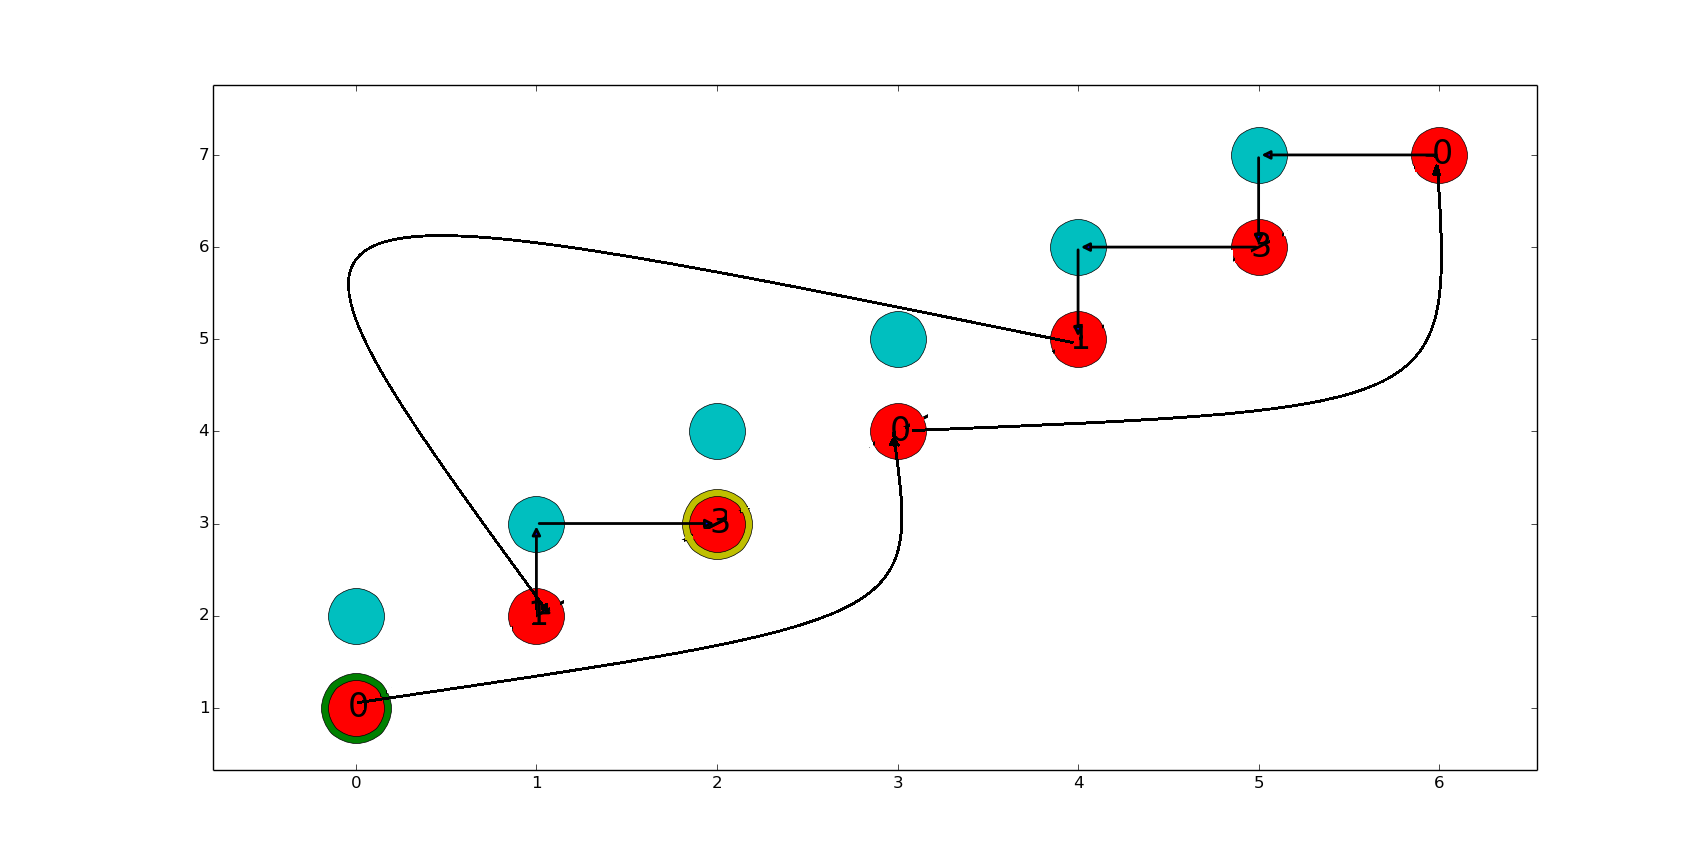
\includegraphics[scale=0.3]{./EJ3/gym0goloso.png}\\
 {            \textit{Soluci\'on Golosa}}
  \end{center}
  \vspace*{0.3cm}

\vspace*{0.3cm} \vspace*{0.3cm}
  \begin{center}
 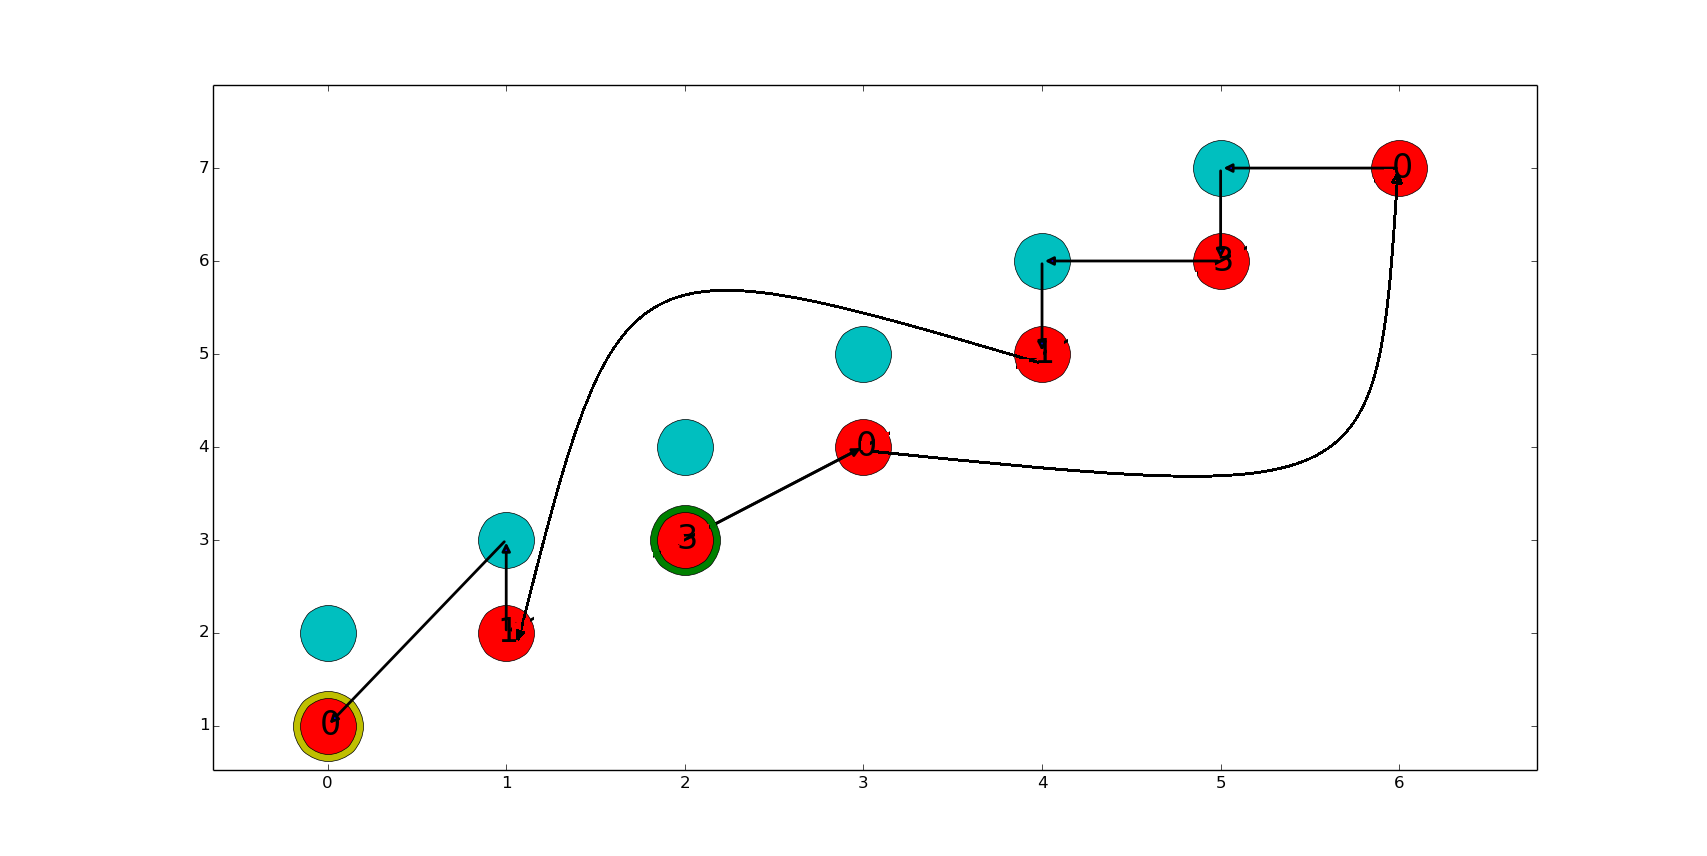
\includegraphics[scale=0.3]{./EJ3/gym0swap.png}\\
 {            \textit{Soluci\'on SWAP}}
  \end{center}
  \vspace*{0.3cm}

\vspace*{0.3cm} \vspace*{0.3cm}
  \begin{center}
 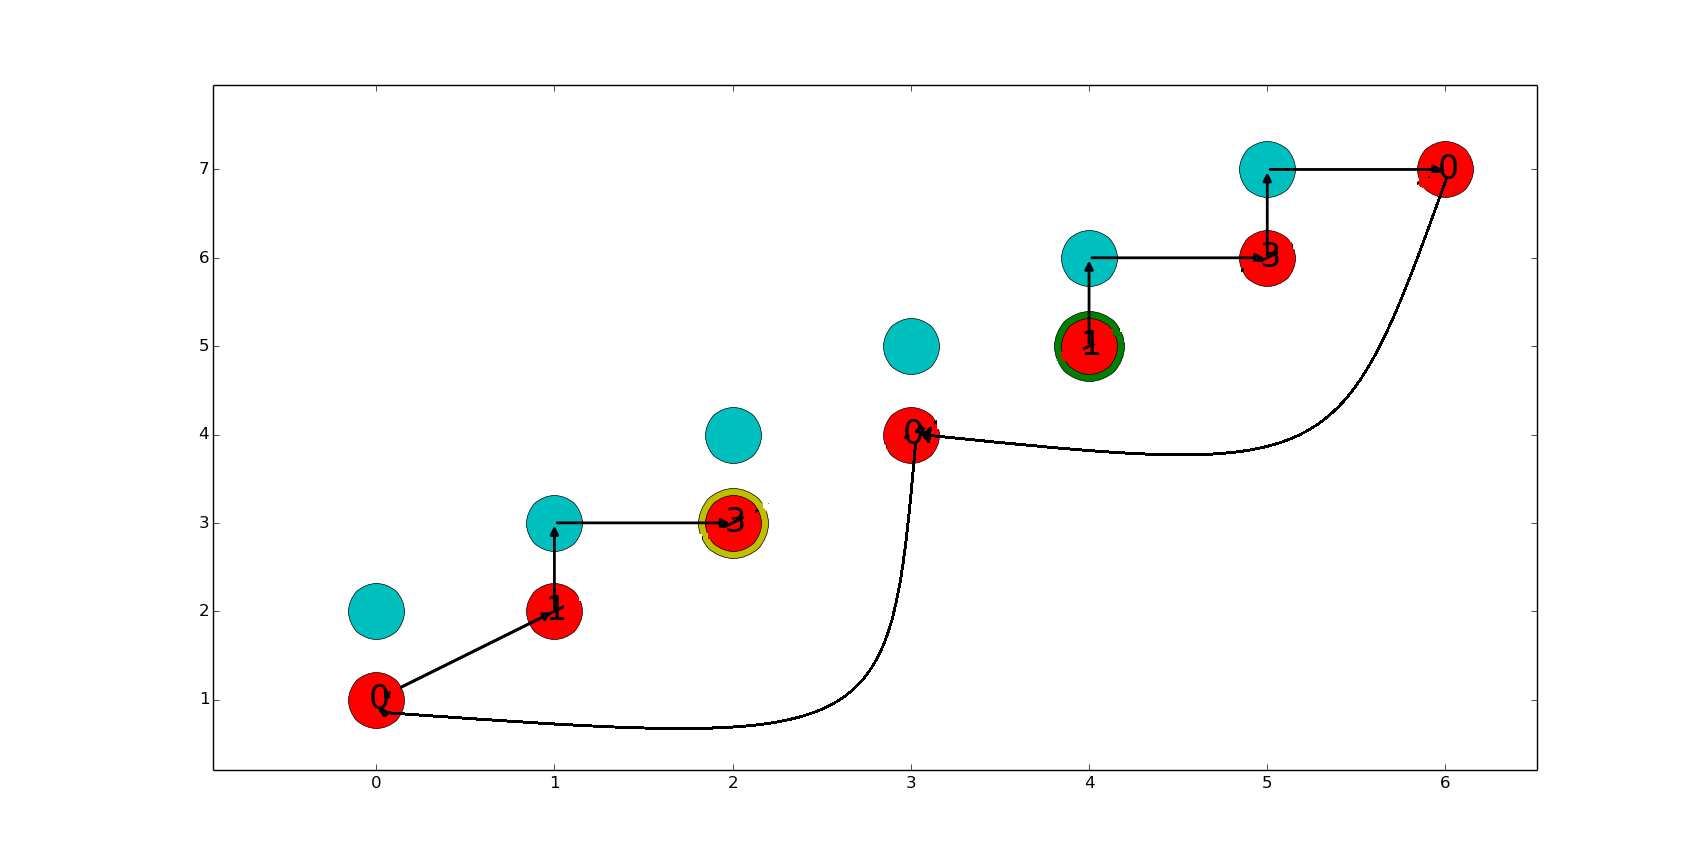
\includegraphics[scale=0.3]{./EJ3/gym02opt.png}\\
 {            \textit{Soluci\'on 2-OPT}}
  \end{center}
  \vspace*{0.3cm}

\vspace*{0.3cm} \vspace*{0.3cm}
  \begin{center}
 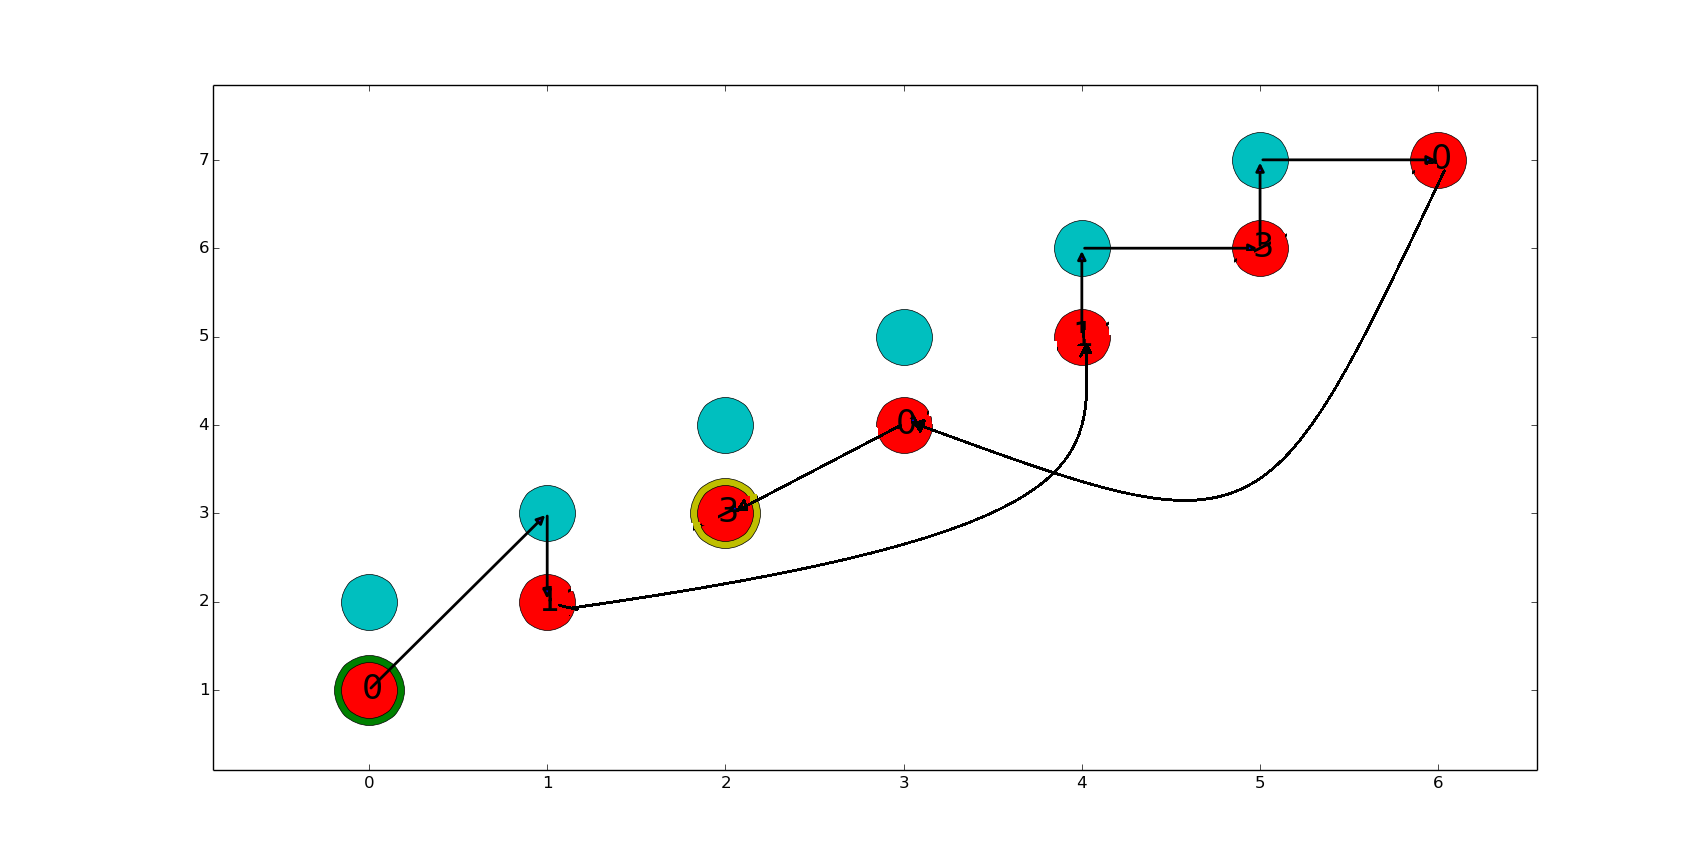
\includegraphics[scale=0.3]{./EJ3/gym03opt.png}\\
 {            \textit{Soluci\'on 3-OPT}}
  \end{center}
  \vspace*{0.3cm}
  
Para la comparación entre algoritmos, se comparará conjuntamente el tiempo de ejecución con la calidad de la solución. Para esta última tendremos en cuenta que los algoritmos, de devolver un resultado, será válido: esto quiere decir que cuanto menor distancia recorran en las soluciones, mejor serán las mismas:

\vspace*{0.3cm} \vspace*{0.3cm}
  \begin{center}
 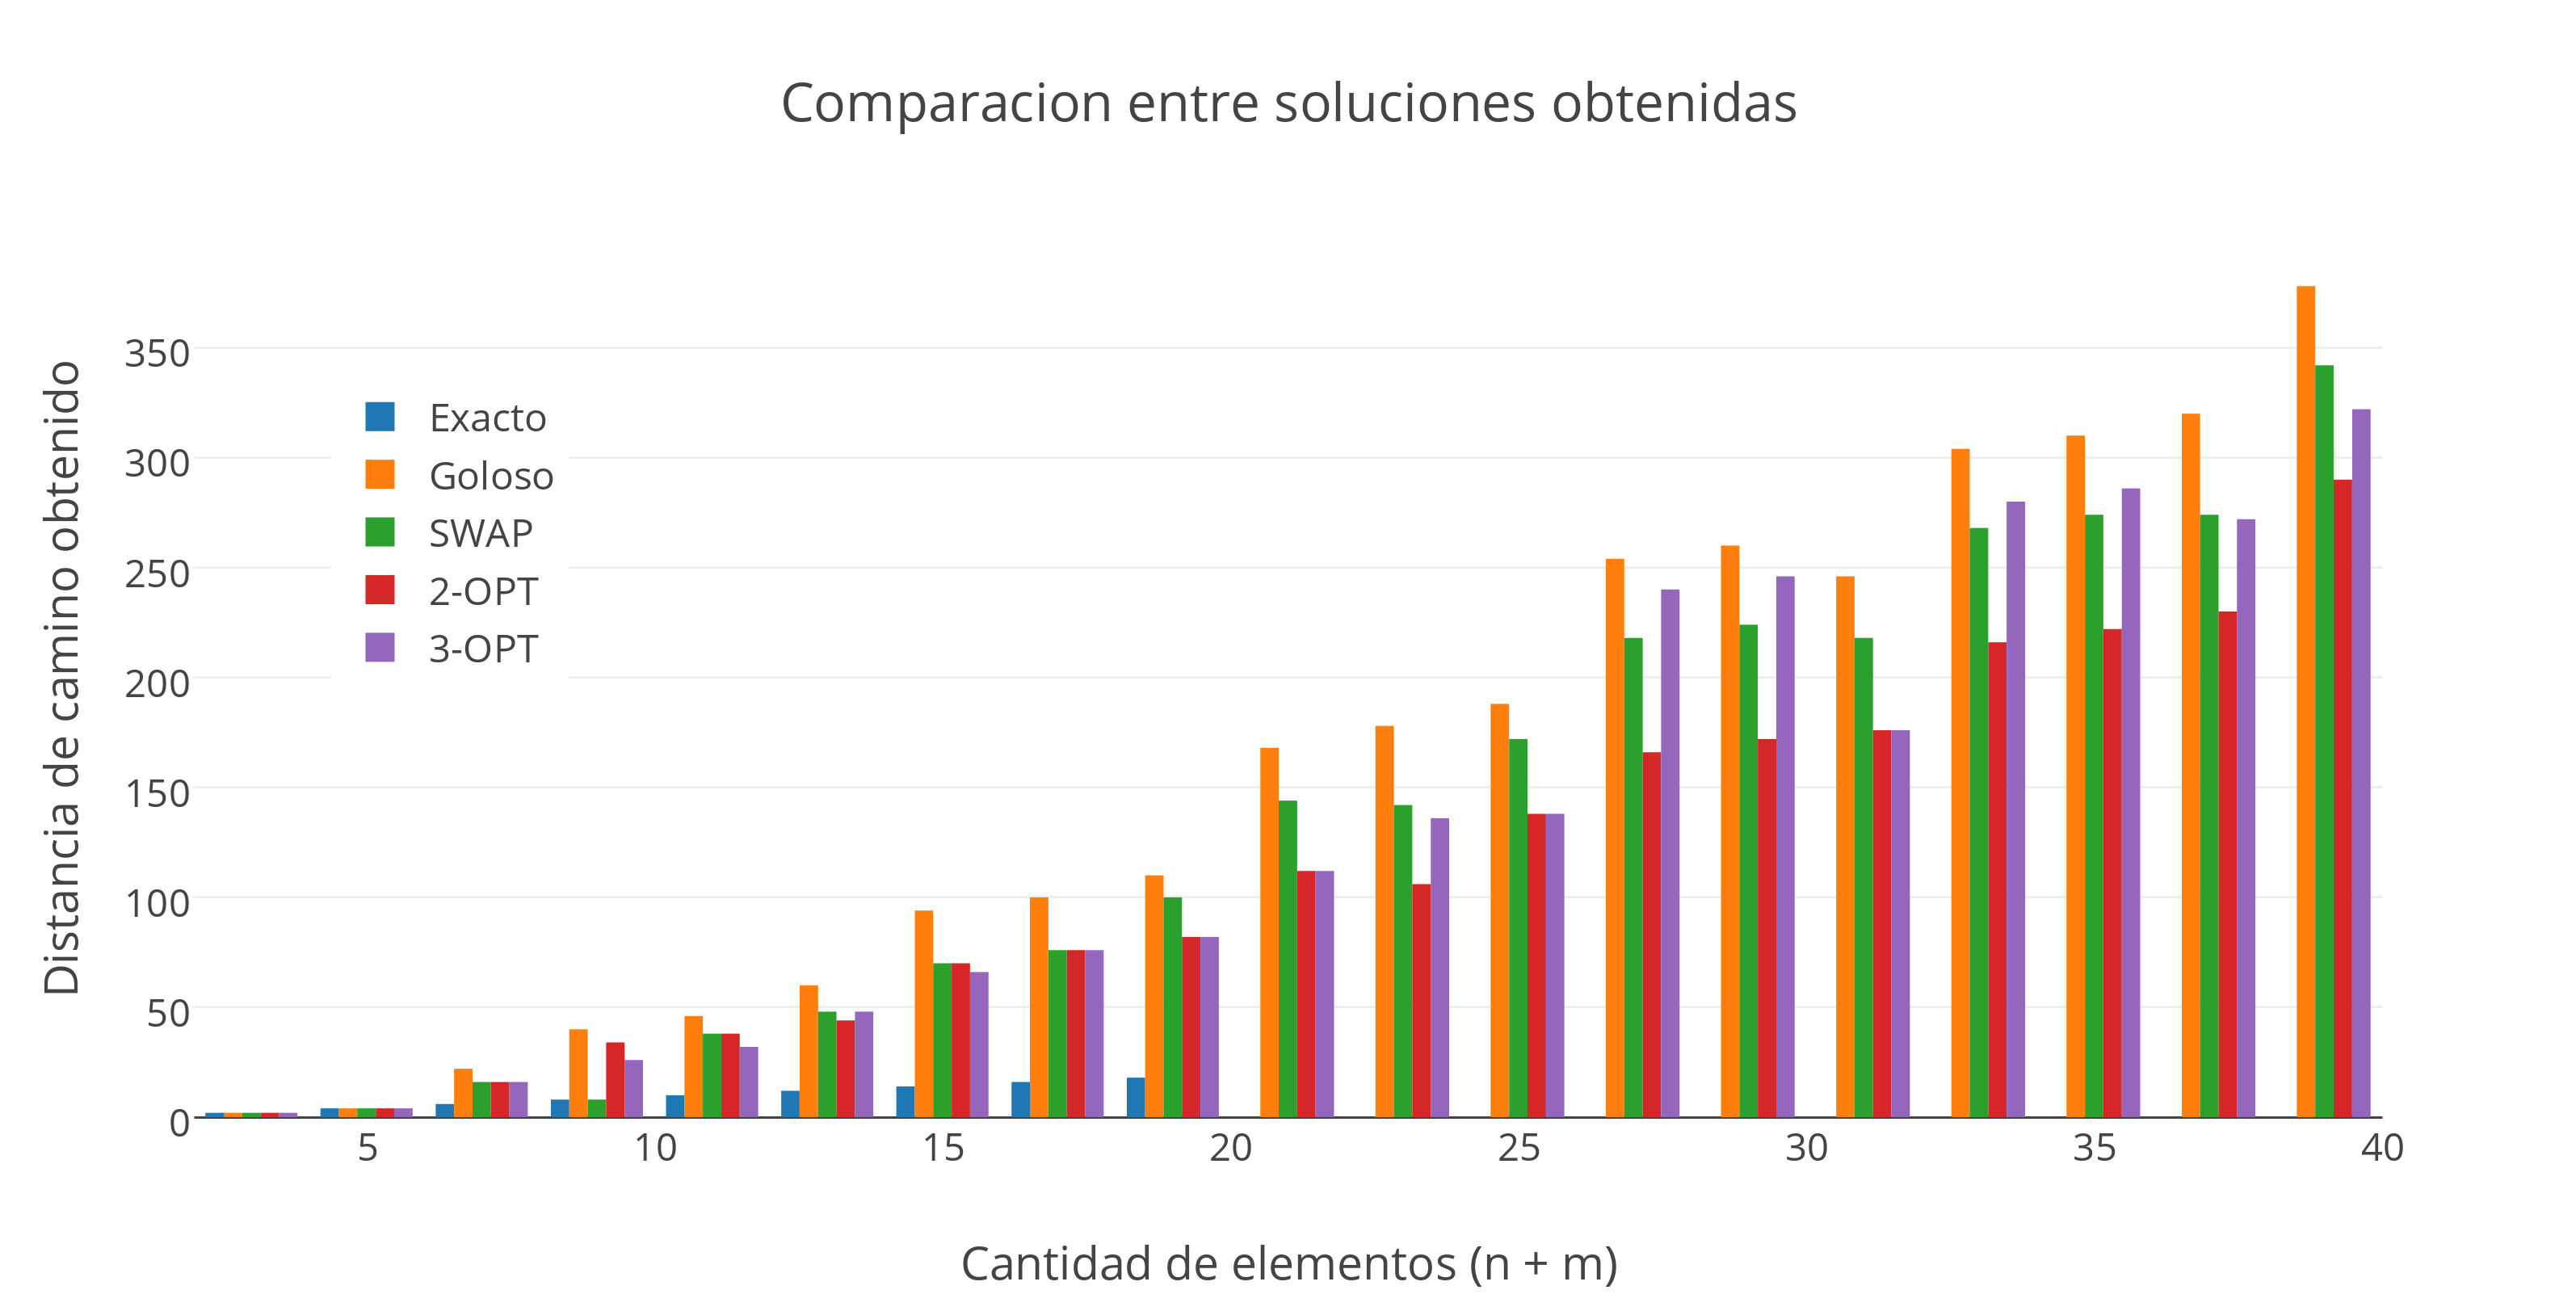
\includegraphics[scale=0.5]{./EJ3/comparacionbusquedaslocalessoluciongym0.png}\\
 {            \textit{Gráfico \ 3.1 - Búsquedas locales sobre Familia 4}}
  \end{center}
  \vspace*{0.3cm}
  
En cuanto a tiempo insumido vemos lo siguiente:

\vspace*{0.3cm} \vspace*{0.3cm}
  \begin{center}
 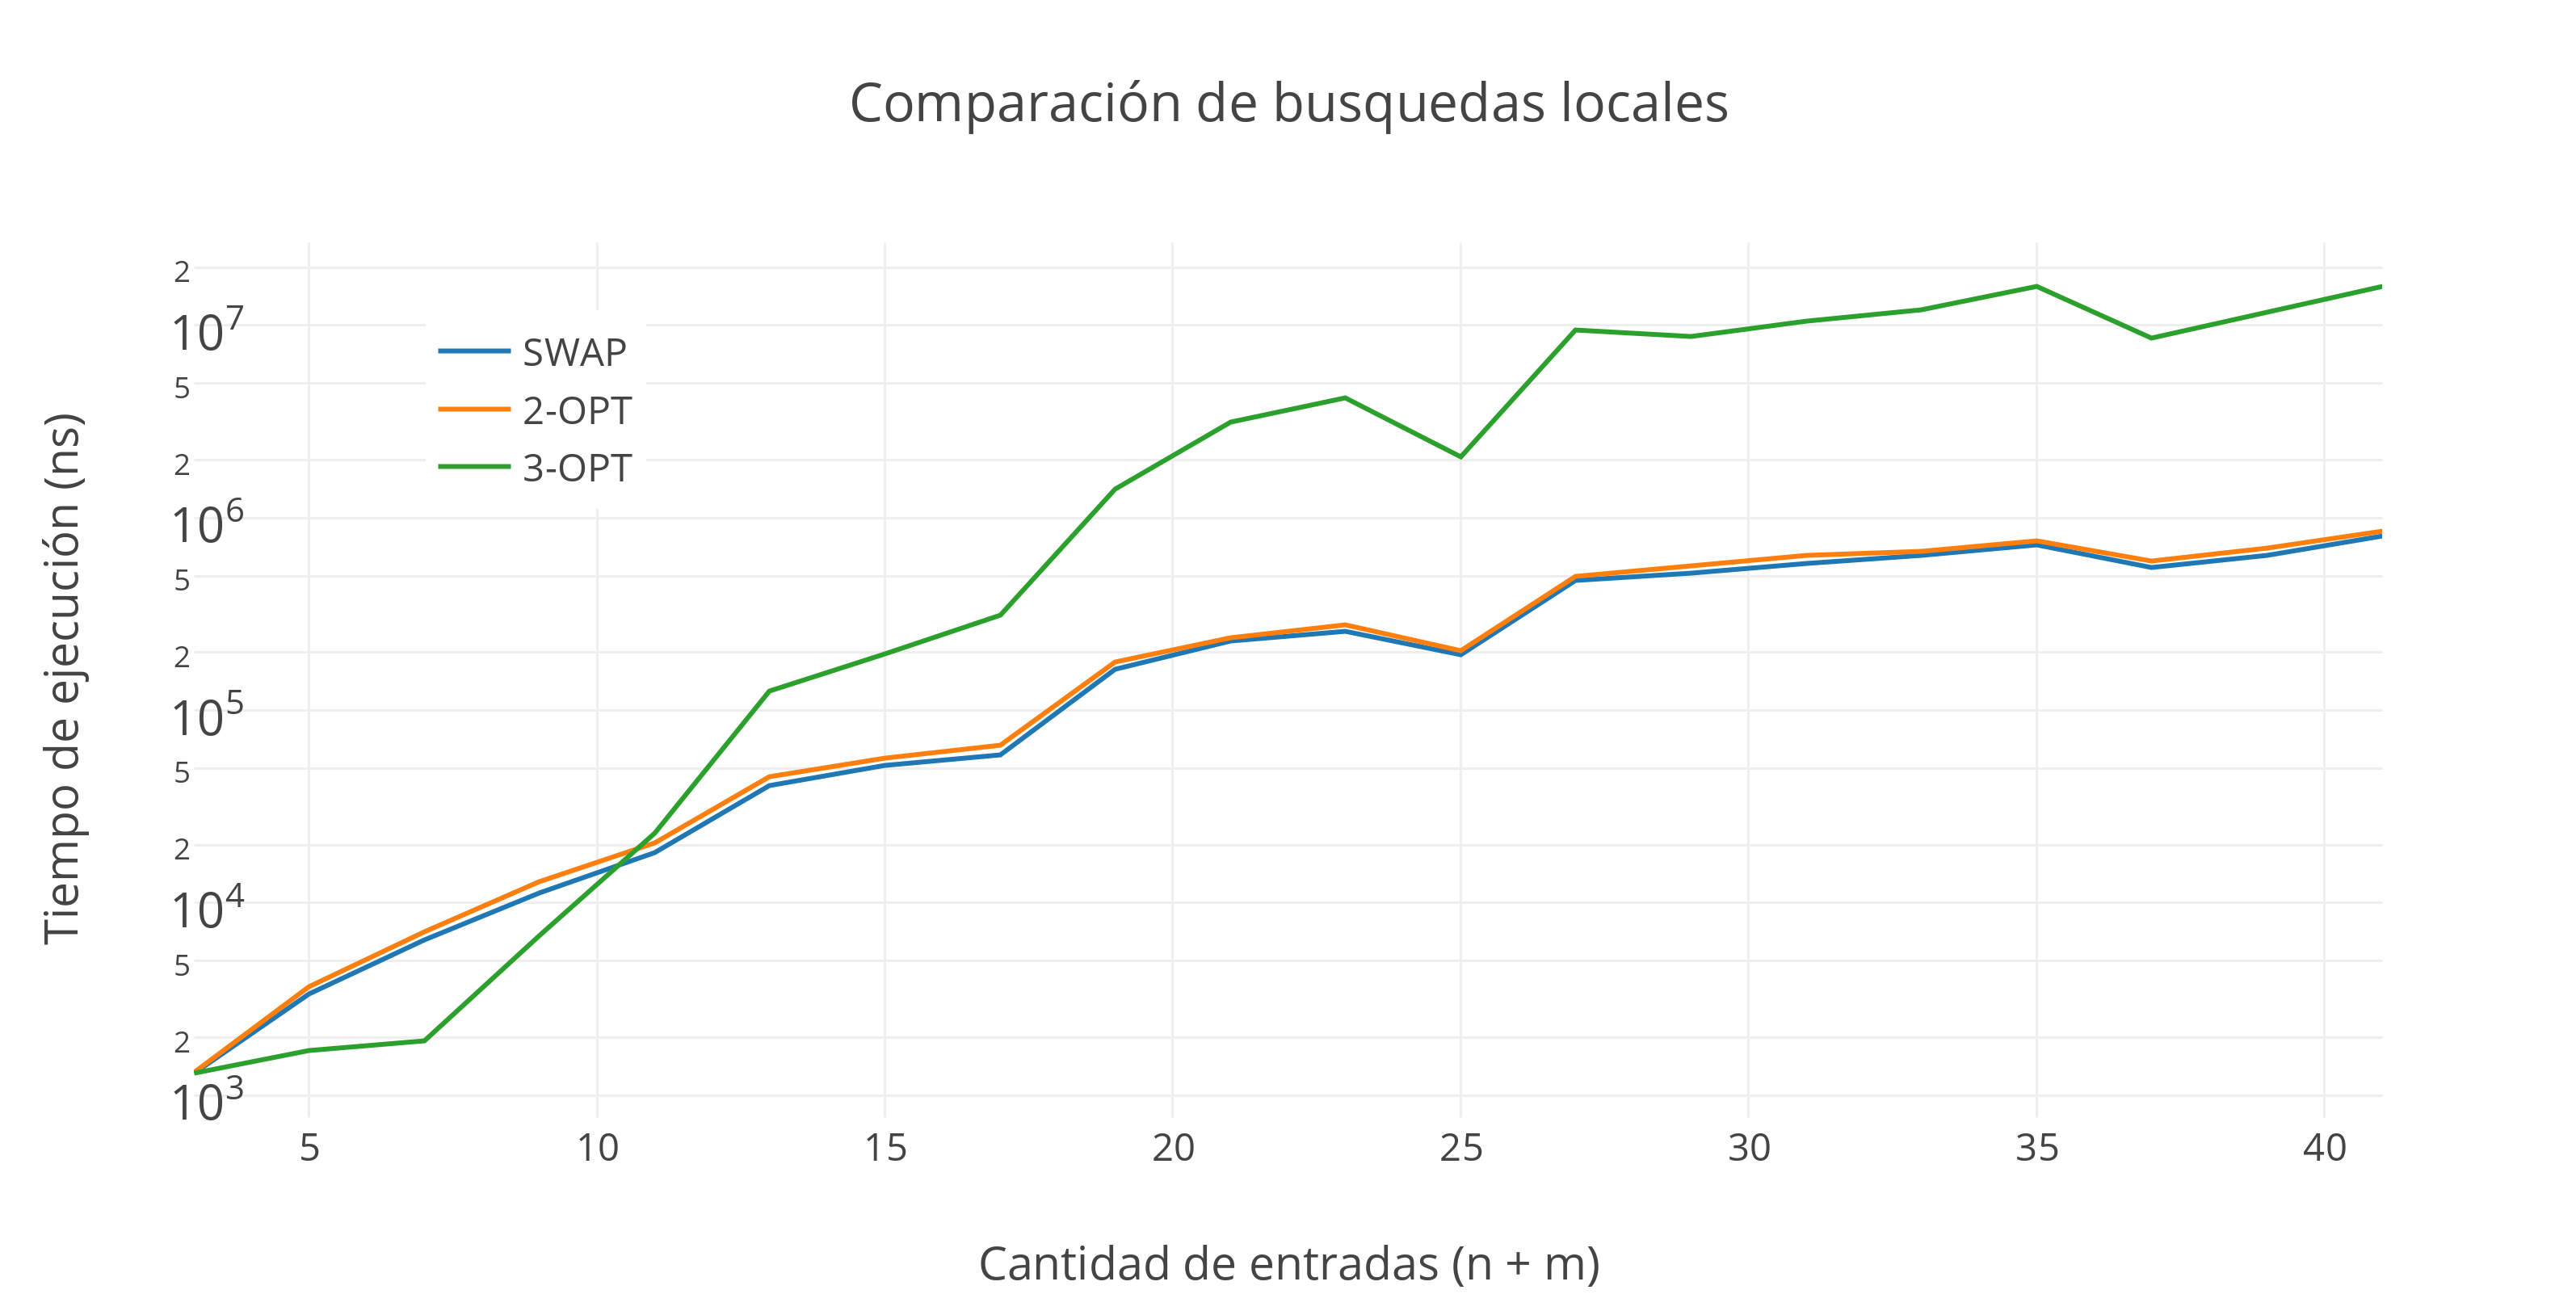
\includegraphics[scale=0.5]{./EJ3/comparacionbusquedaslocalesgym0.png}\\
 {            \textit{Gráfico \ 3.2 - Búsquedas locales sobre Familia 4}}
  \end{center}
  \vspace*{0.3cm}

En este caso, el tiempo de ejecuci\'on de SWAP y 2-OPT tienen un desempeño temporal muy similar, no obstante, al comparar la calidad de solución, 2-OPT posee los mejores resultados. En cuanto a la variante 3-OPT: no solo genera peores soluciones, sino que tarda mucho más que las otras dos búsquedas para instancias con muchas pokeparadas y gimnasios y la mejora no es significativa para entradas pequeñas, lo que puede inducir a que para esta familia de casos no sea conveniente utilizar 3-OPT.

Como se explicó anteriormente, que una búsqueda local K-OPT no genere buenos resultados, siempre está relacionado con una entrada en particular y no al hecho de que la búsqueda en si misma sea mala. Es posible que partiendo de una solución golosa, la mejor solución se encuentre haciendo determinado número de movimiento de aristas y no otro. Encontrar una explicación al poque sucede esto para una entrada particular, requiere indagar fuertemente en las propiedades de la entrada, como la posicion de las pokeparadas y aristas que conforman la solución a optimizar, lo cual puede no ser sencillo.\\

\subsubsection*{Familia 6}

Mostraremos una instancia de este conjunto iniciando por el camino obtenido a partir de la soluci\'on golosa y como es modificado por cada heuristica, para luego, comparar todo el conjunto en cuesti\'on:

\vspace*{0.3cm} \vspace*{0.3cm}
  \begin{center}
 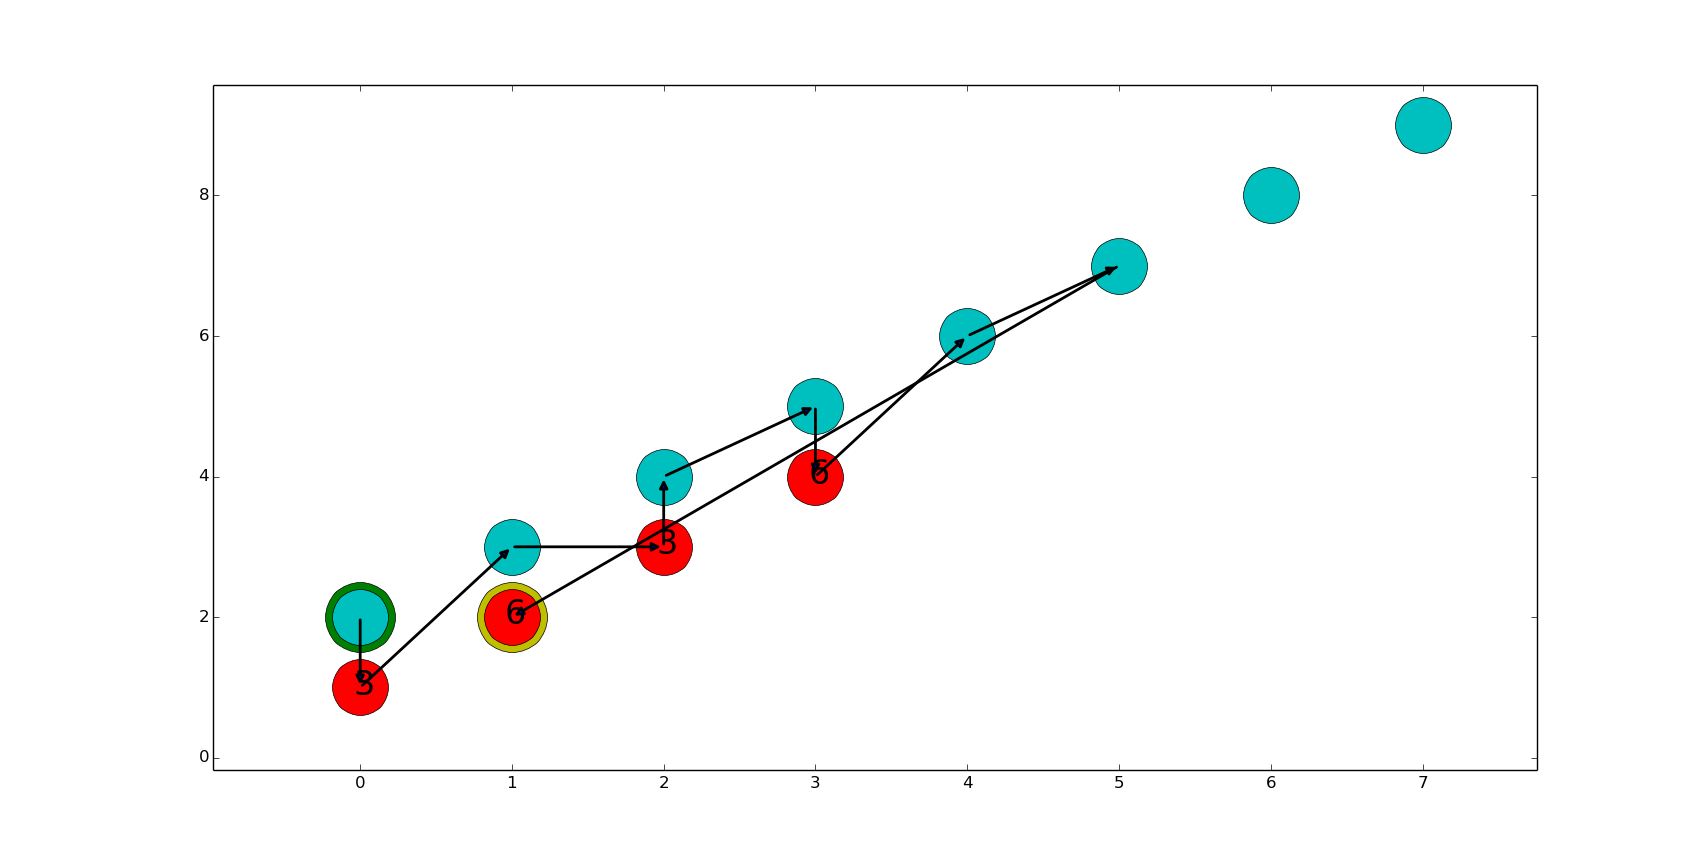
\includegraphics[scale=0.3]{./EJ3/sinOrdengoloso.png}\\
 {            \textit{Soluci\'on Golosa}}
  \end{center}
  \vspace*{0.3cm}

\vspace*{0.3cm} \vspace*{0.3cm}
  \begin{center}
 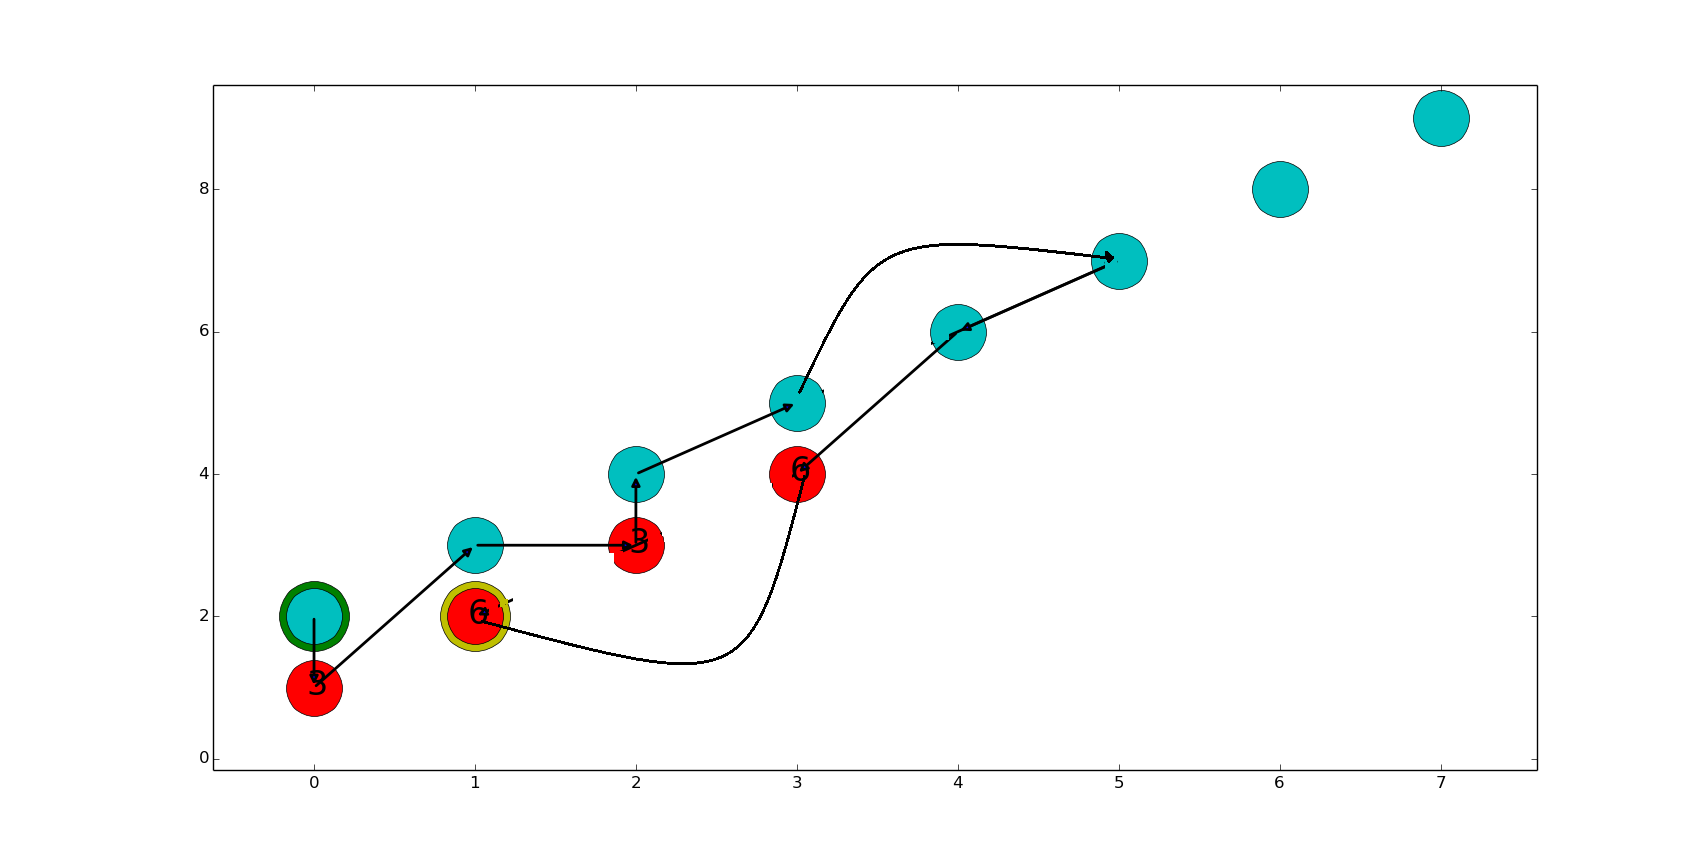
\includegraphics[scale=0.3]{./EJ3/sinOrdenswap.png}\\
 {            \textit{Soluci\'on SWAP}}
  \end{center}
  \vspace*{0.3cm}

\vspace*{0.3cm} \vspace*{0.3cm}
  \begin{center}
 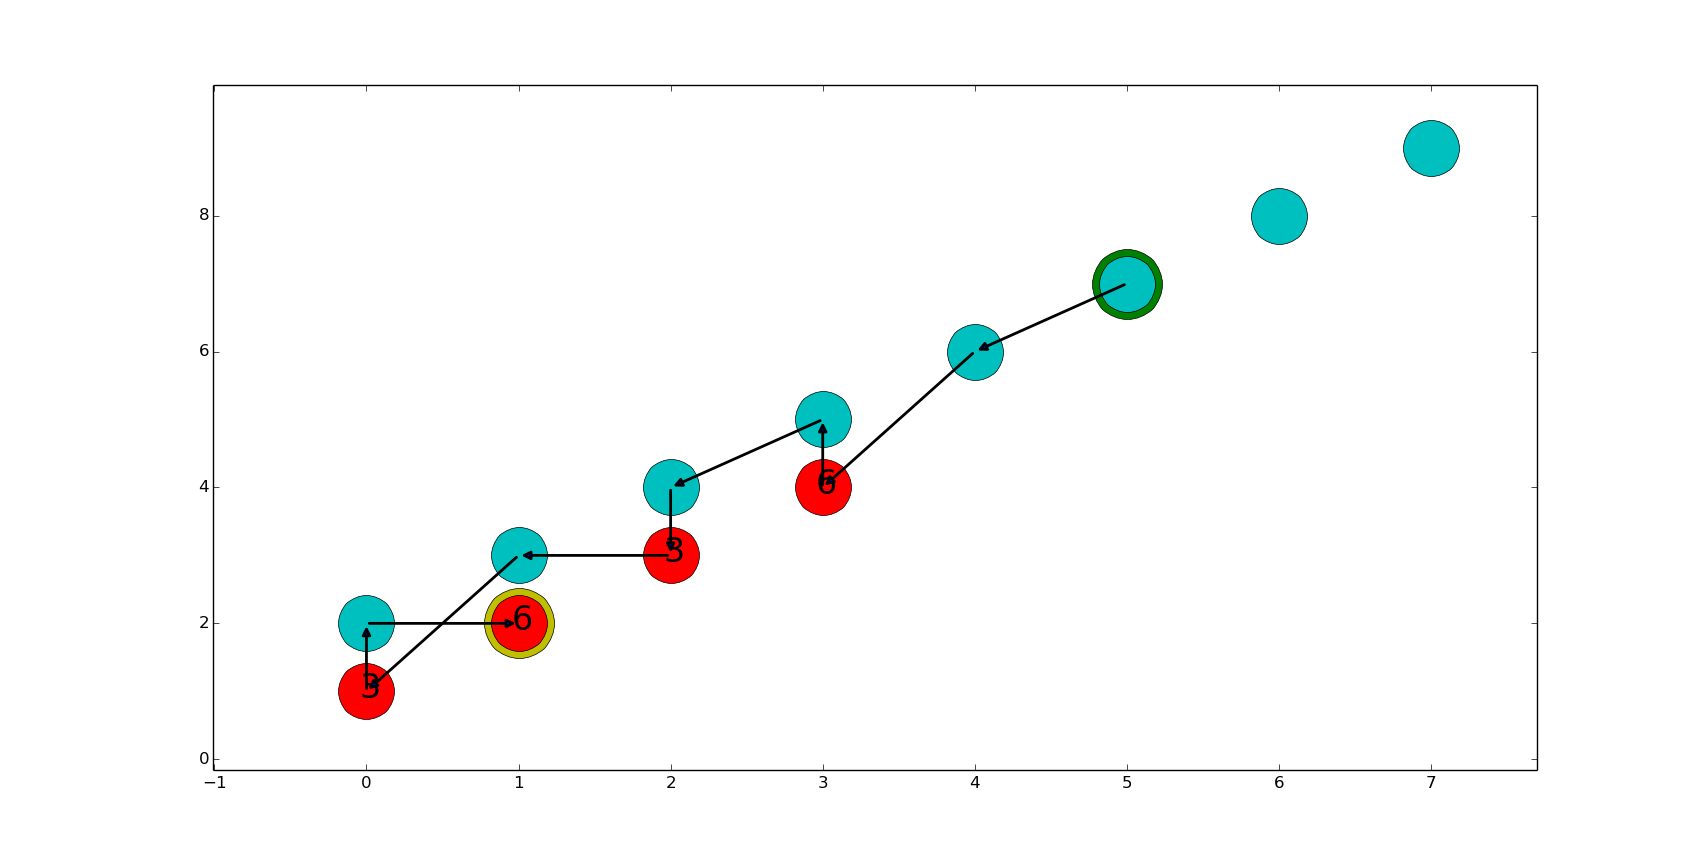
\includegraphics[scale=0.3]{./EJ3/sinOrden2opt.png}\\
 {            \textit{Soluci\'on 2-OPT}}
  \end{center}
  \vspace*{0.3cm}


\vspace*{0.3cm} \vspace*{0.3cm}
  \begin{center}
 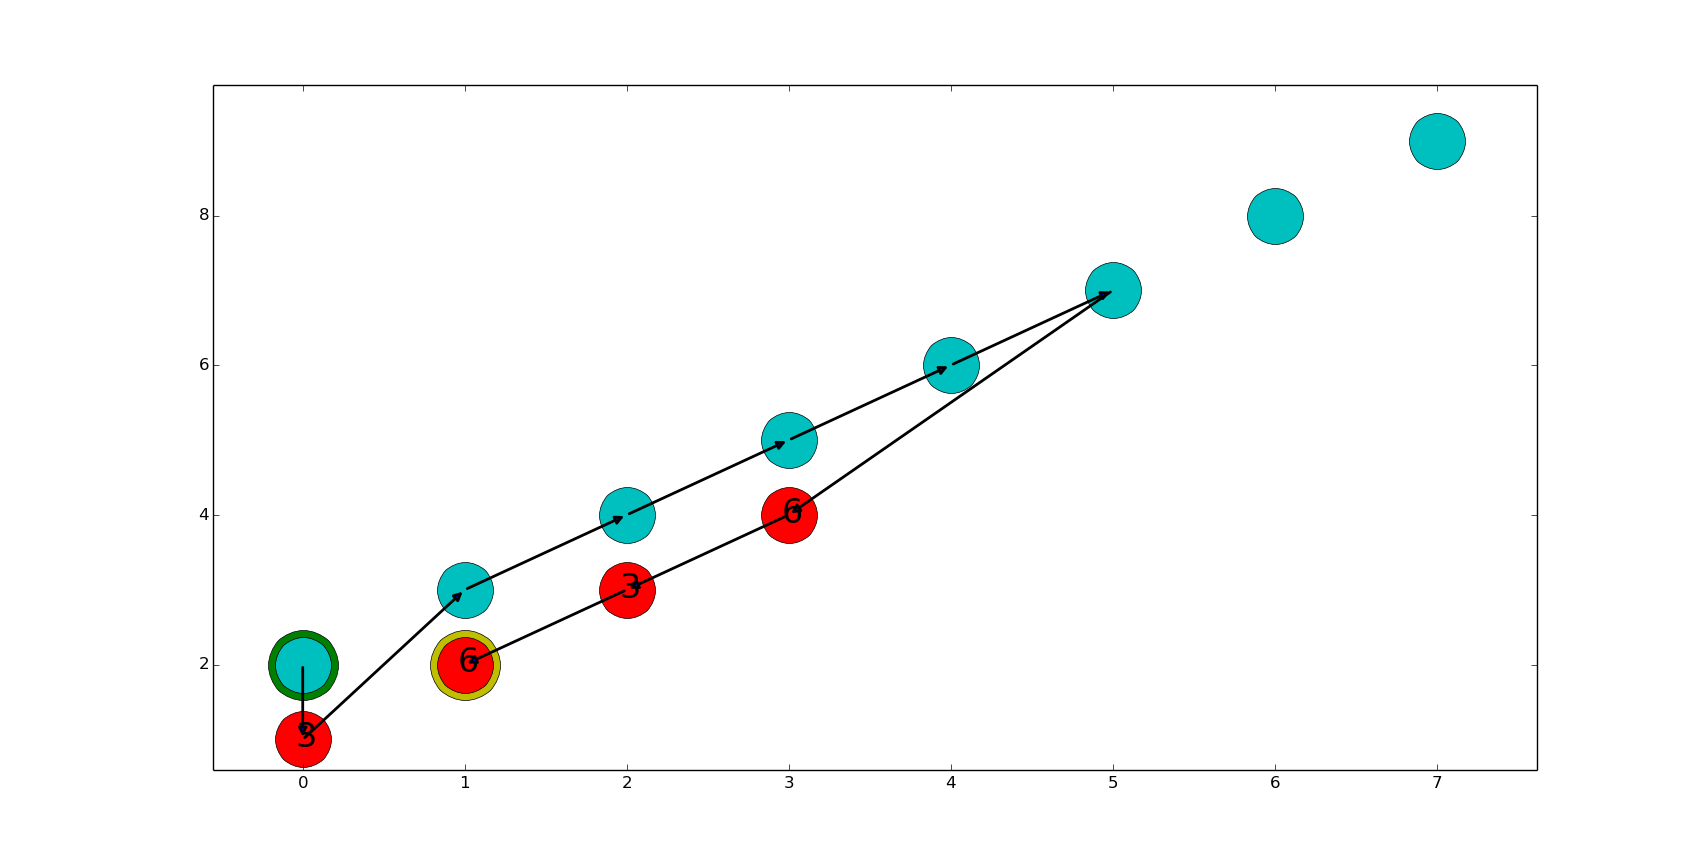
\includegraphics[scale=0.3]{./EJ3/sinOrden3opt.png}\\
 {            \textit{Soluci\'on 3-OPT}}
  \end{center}
  \vspace*{0.3cm}


\vspace*{0.3cm} \vspace*{0.3cm}
  \begin{center}
 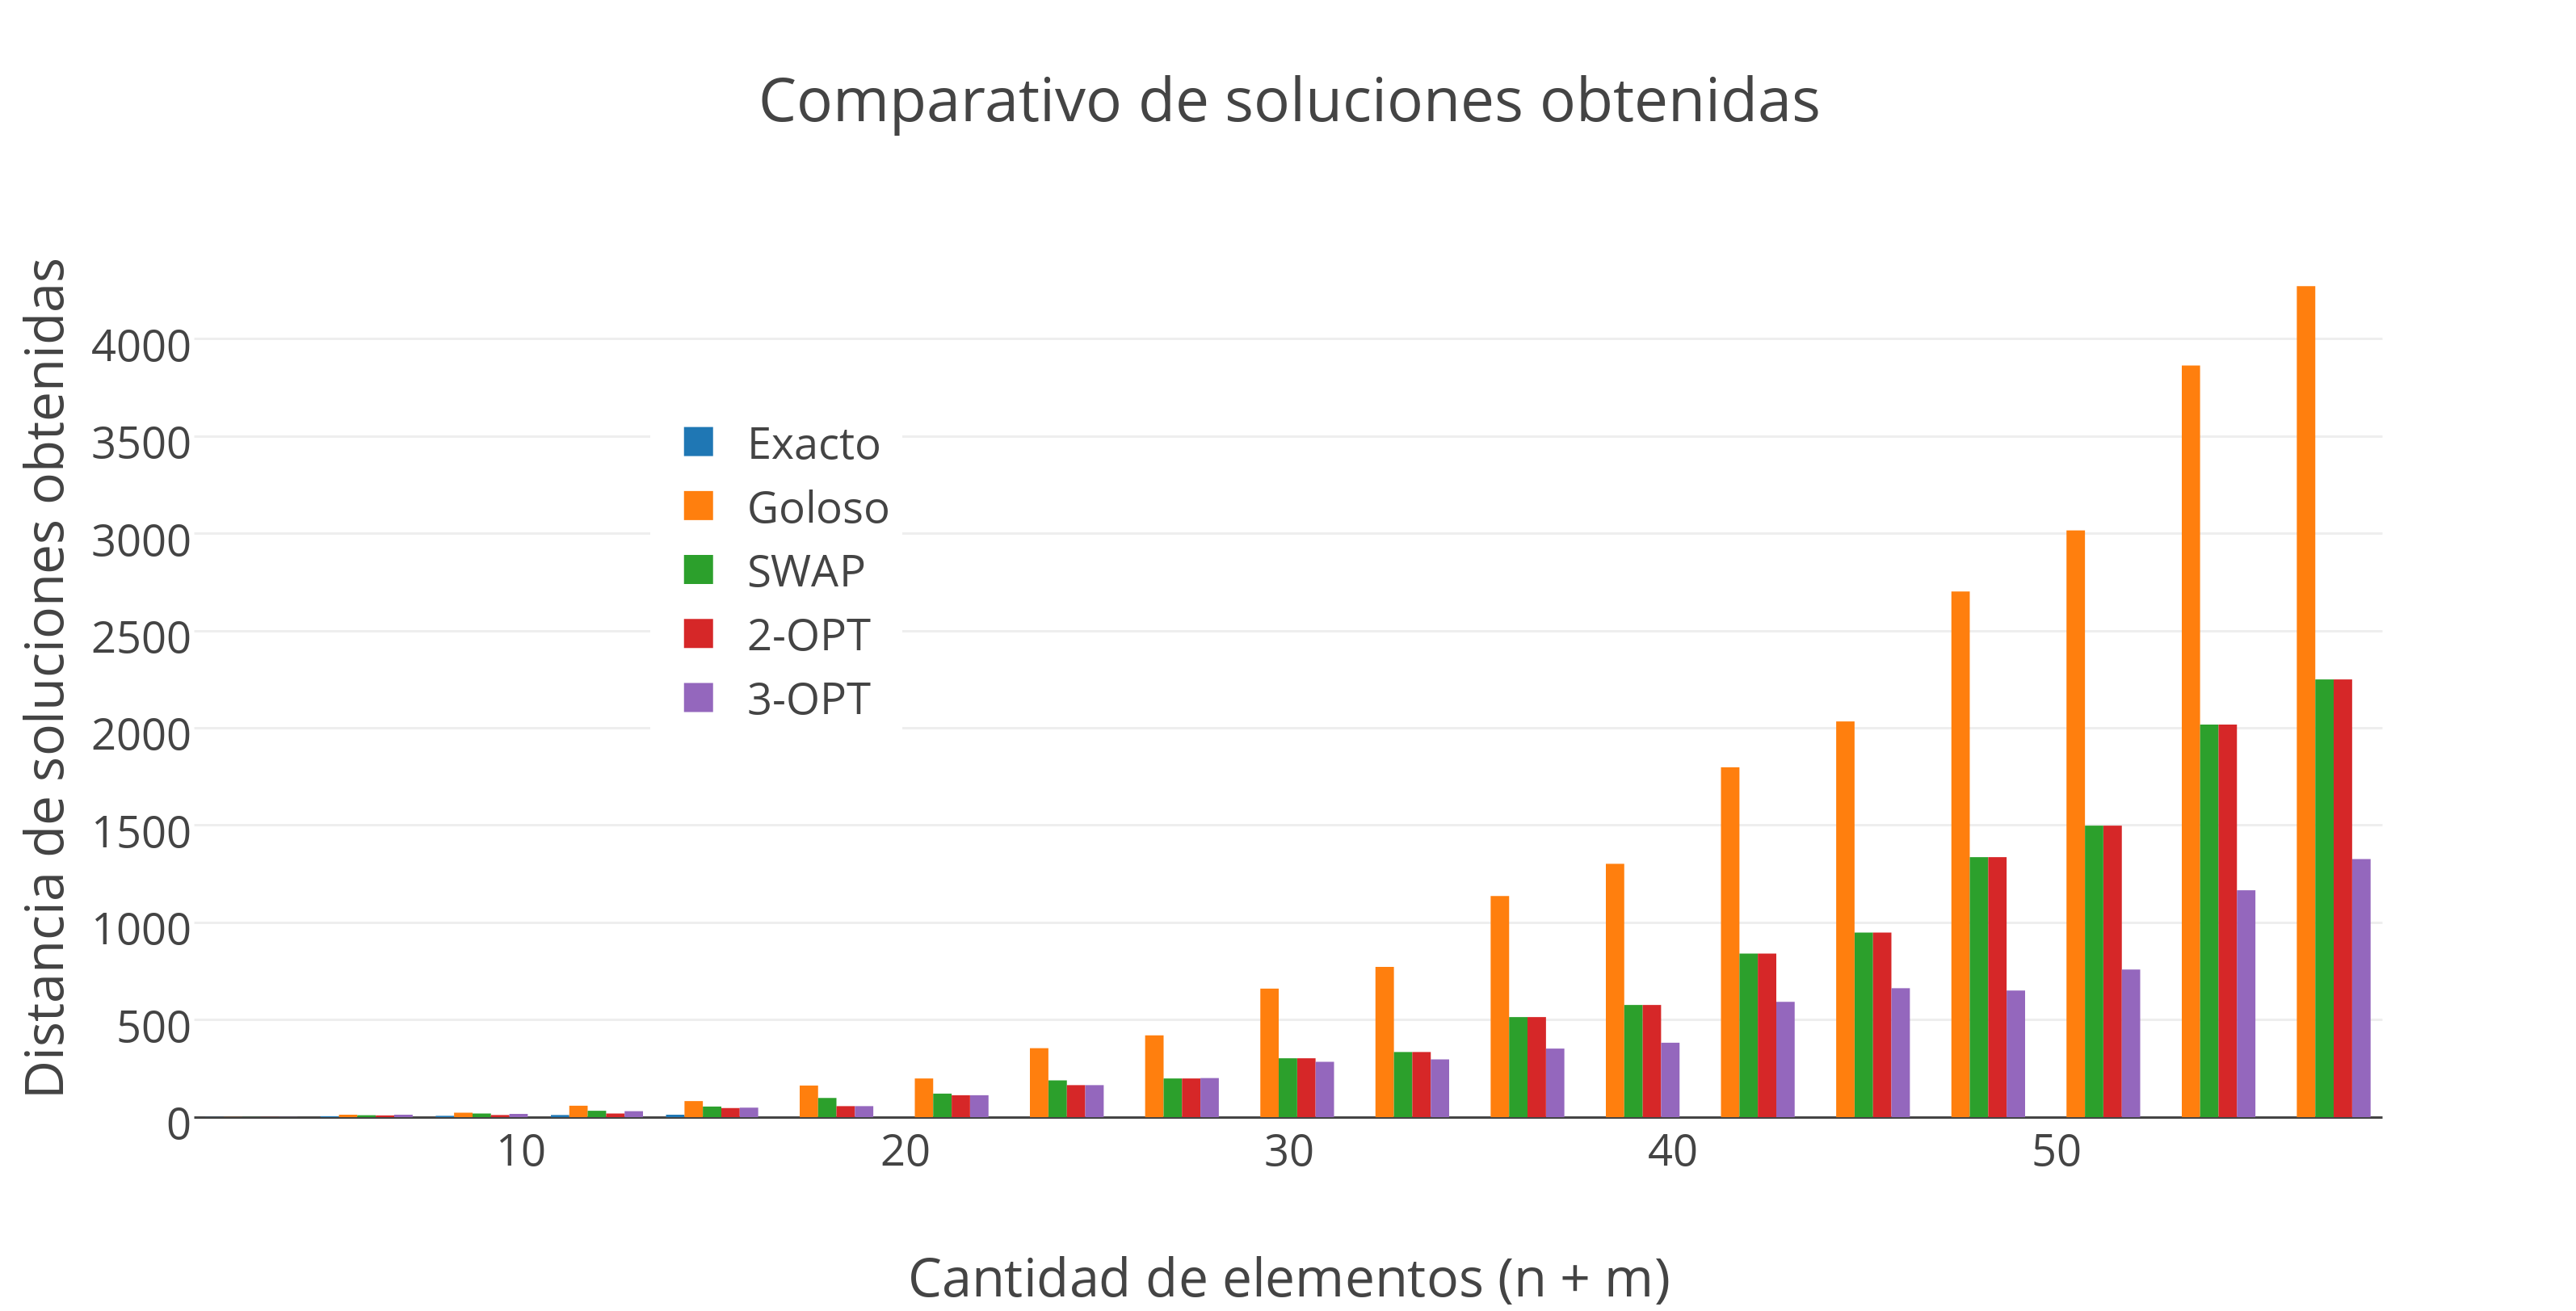
\includegraphics[scale=0.5]{./EJ3/comparacionbusquedaslocalessolucionsinorden.png}\\
 {            \textit{Gráfico \ 3.4 - Búsquedas locales sobre Familia 6}}
  \end{center}
  \vspace*{0.3cm}


\vspace*{0.3cm} \vspace*{0.3cm}
  \begin{center}
 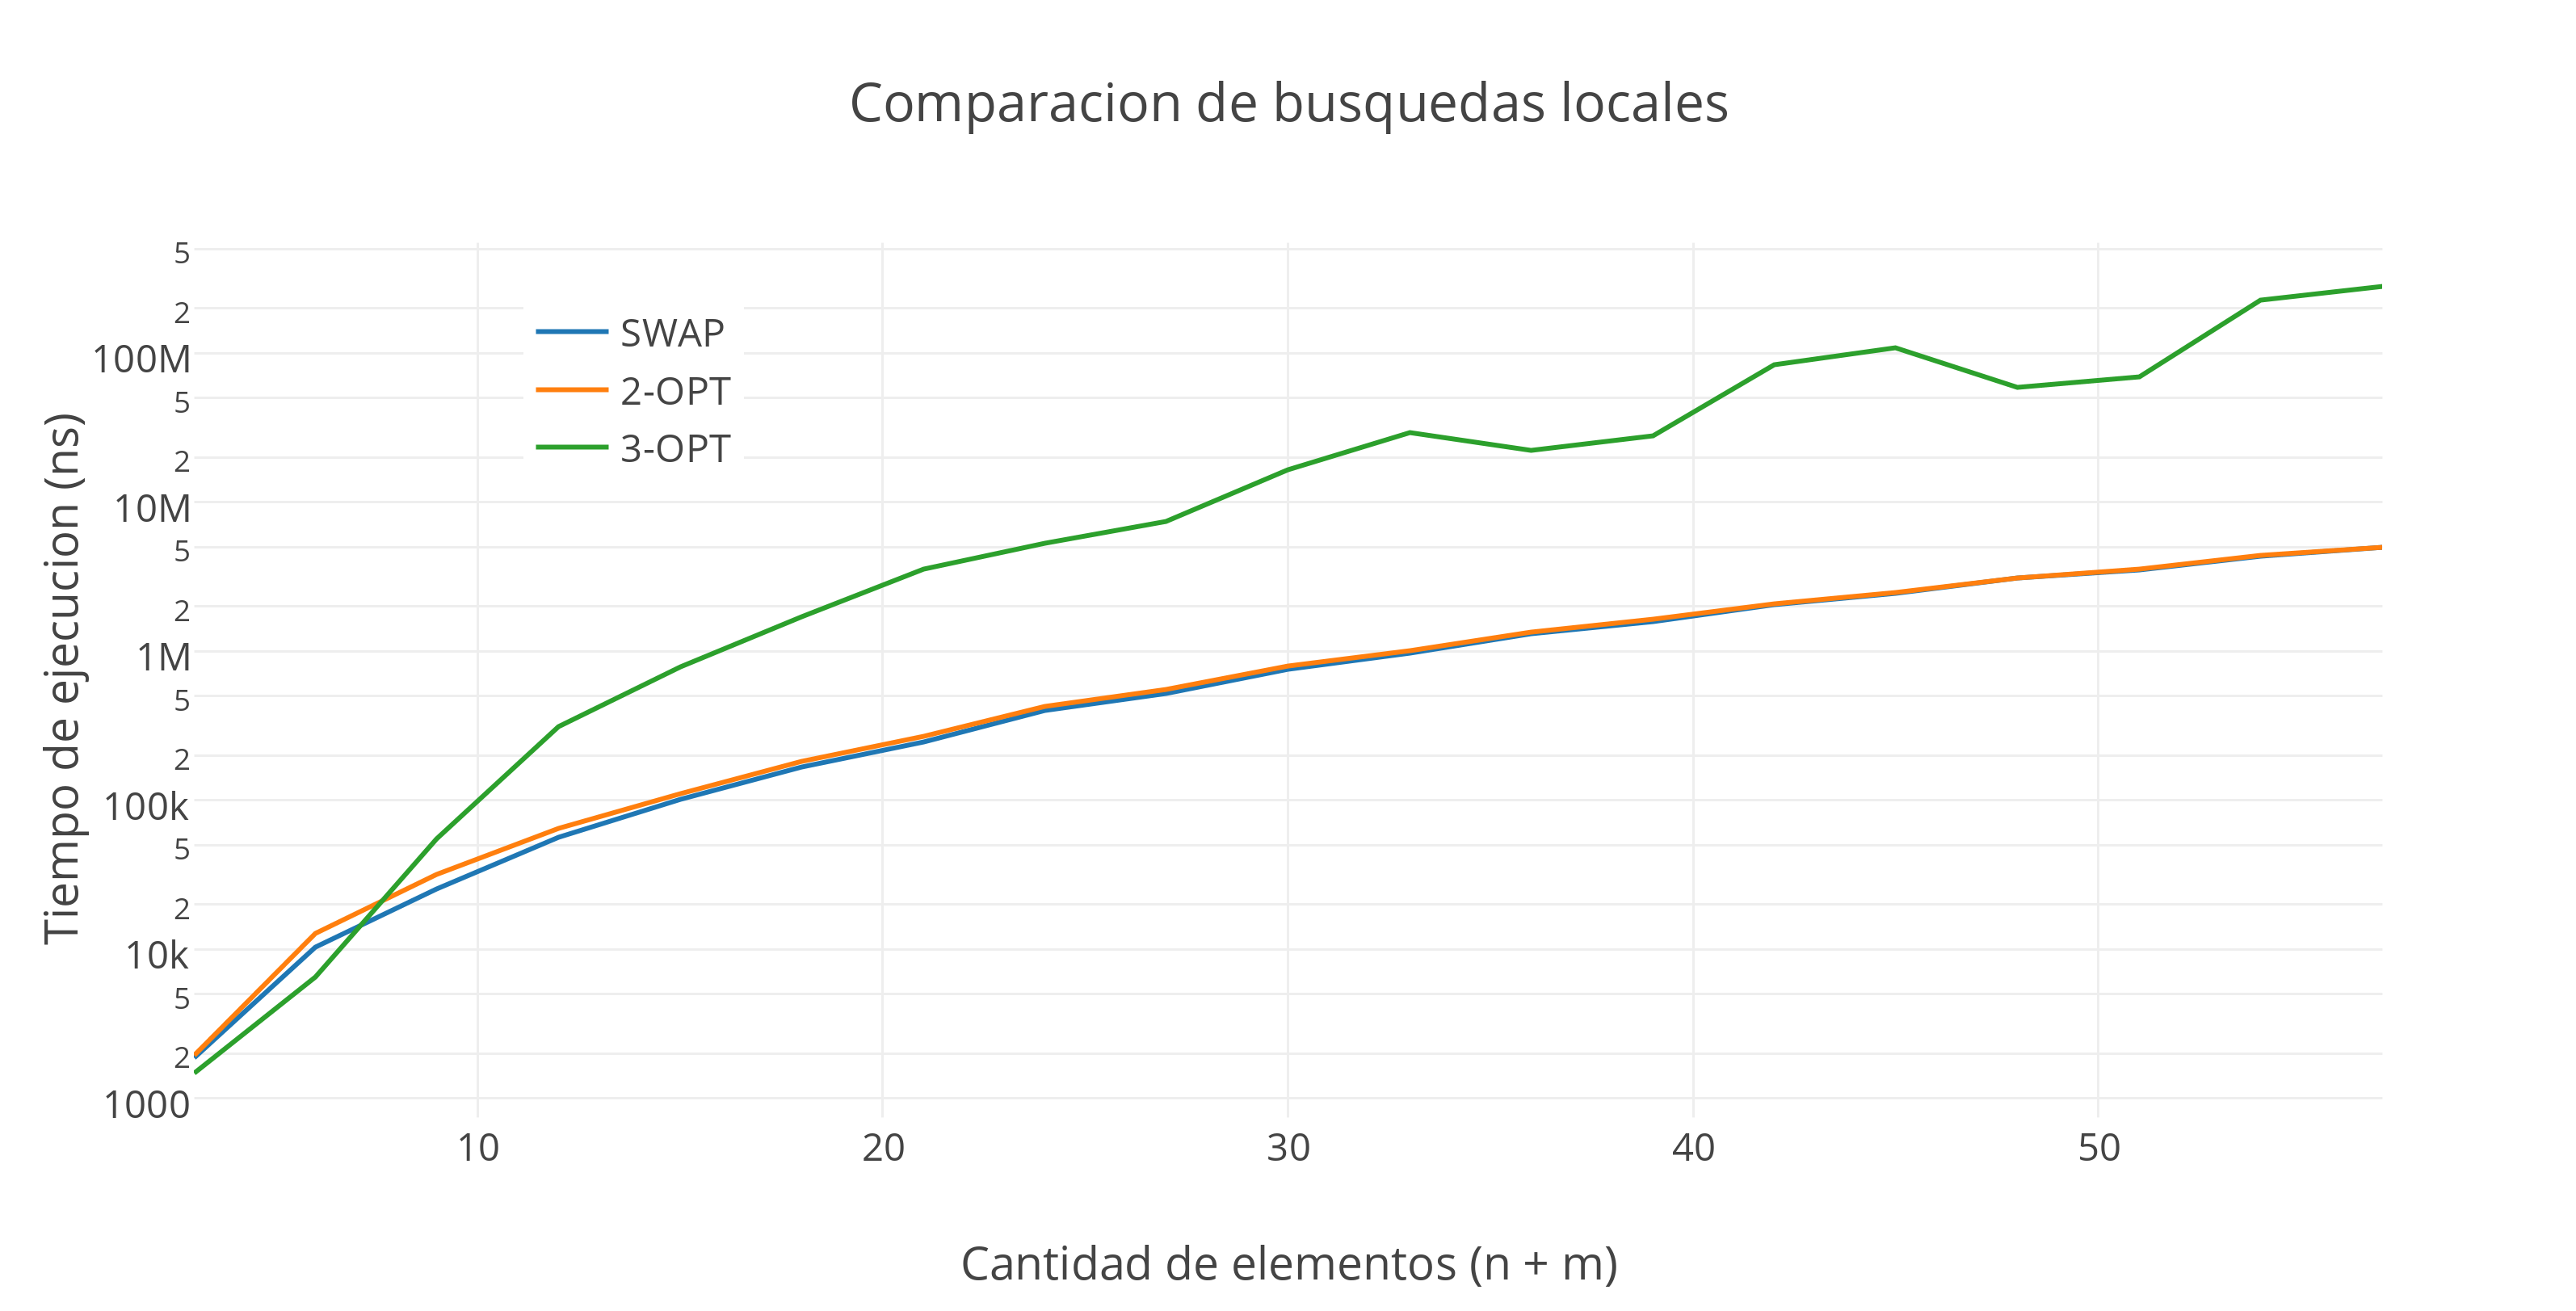
\includegraphics[scale=0.5]{./EJ3/comparacionbusquedaslocalessinorden.png}\\
 {            \textit{Gráfico \ 3.3 - Búsquedas locales sobre Familia 6}}
  \end{center}
  \vspace*{0.3cm}

Comparando los tiempos de ejecución, SWAP es muy similar a 2-OPT y 3-OPT  posee el peor desempeño. Con respecto a la calidad de los resultados, con 3-OPT se obtienen las mejoras más significativas, pero a un costo mayor en tiempo de ejecución, además, las mejoras realizadas por 2-OPT o SWAP pueden considerarse buenas si se tiene en cuenta la diferencia con respecto al goloso, que es aproximadamente del 50$\%$ en todos los casos.

\subsubsection*{Familia 7}

Exhibiremos una instancia de dicha familia comenzando por el camino obtenido por la heur\'istica golosa y como es modificado por las búsquedas locales. Luego, serán comparados los resultados obtenidos de las mediciones:

\vspace*{0.3cm} \vspace*{0.3cm}
  \begin{center}
 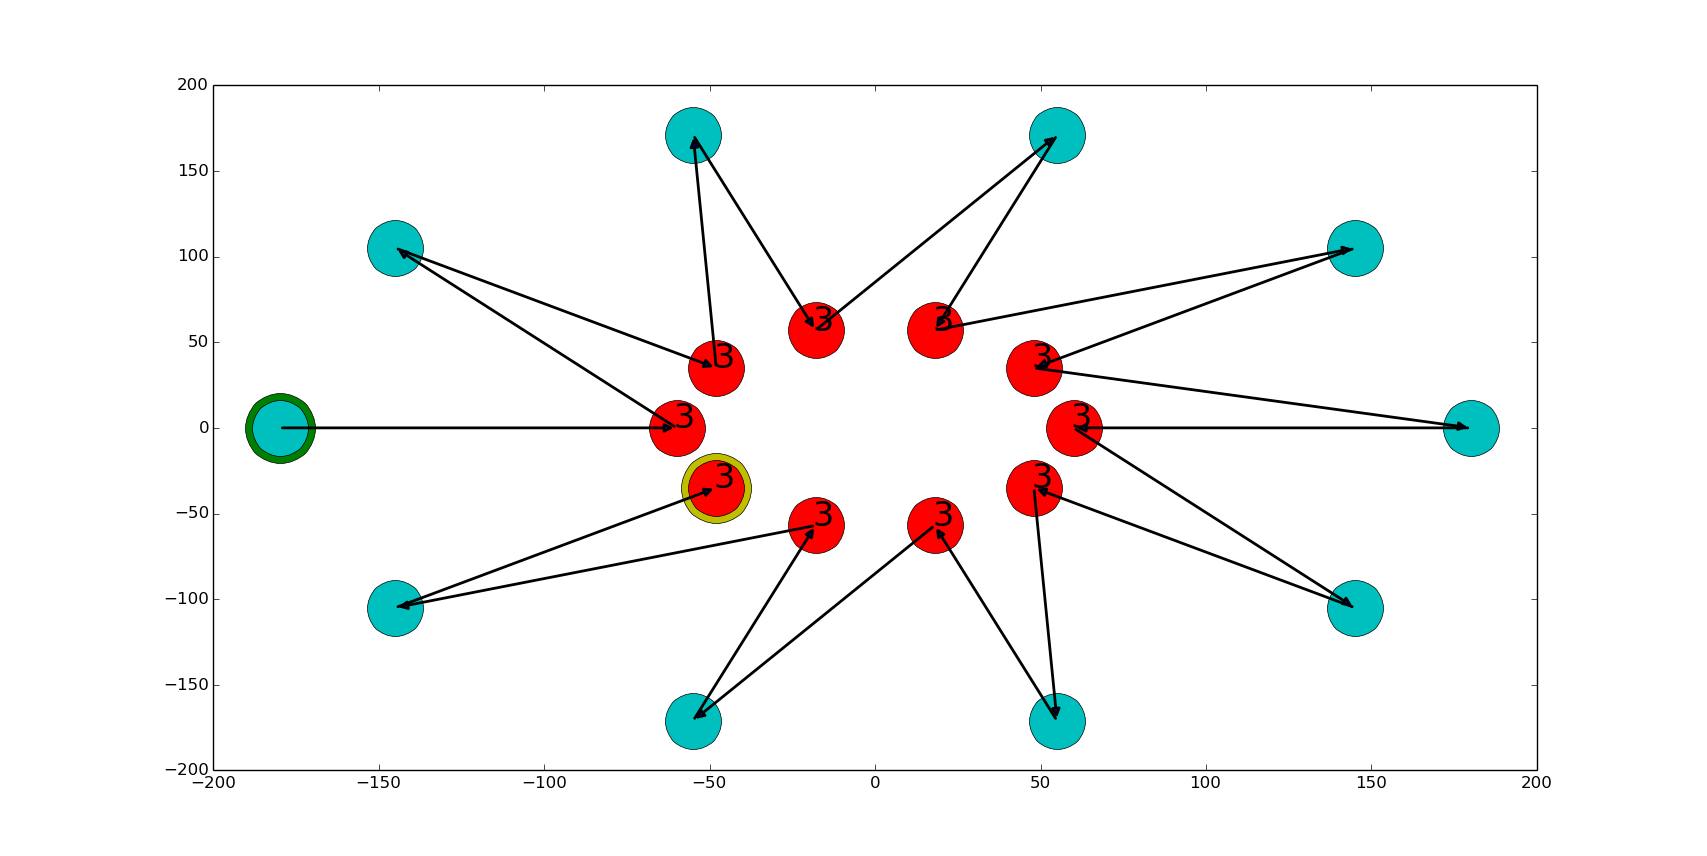
\includegraphics[scale=0.3]{./EJ3/anillosgoloso.png}\\
 {            \textit{Soluci\'on Golosa}}
  \end{center}
  \vspace*{0.3cm}

\vspace*{0.3cm} \vspace*{0.3cm}
  \begin{center}
 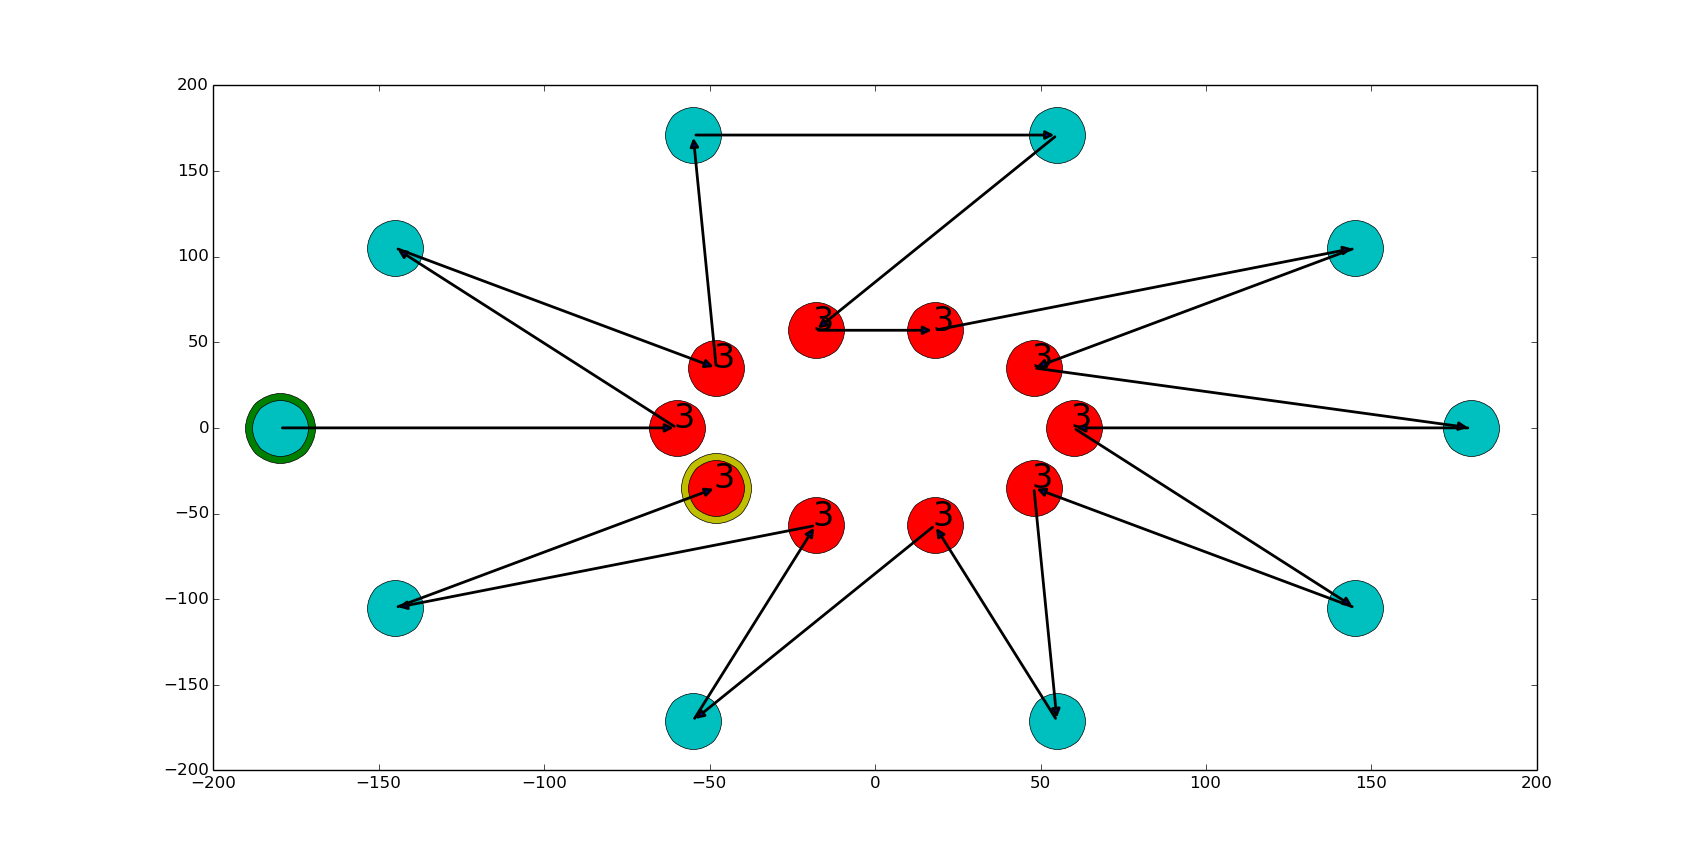
\includegraphics[scale=0.3]{./EJ3/anillosswap.png}\\
 {            \textit{Soluci\'on SWAP}}
  \end{center}
  \vspace*{0.3cm}

\vspace*{0.3cm} \vspace*{0.3cm}
  \begin{center}
 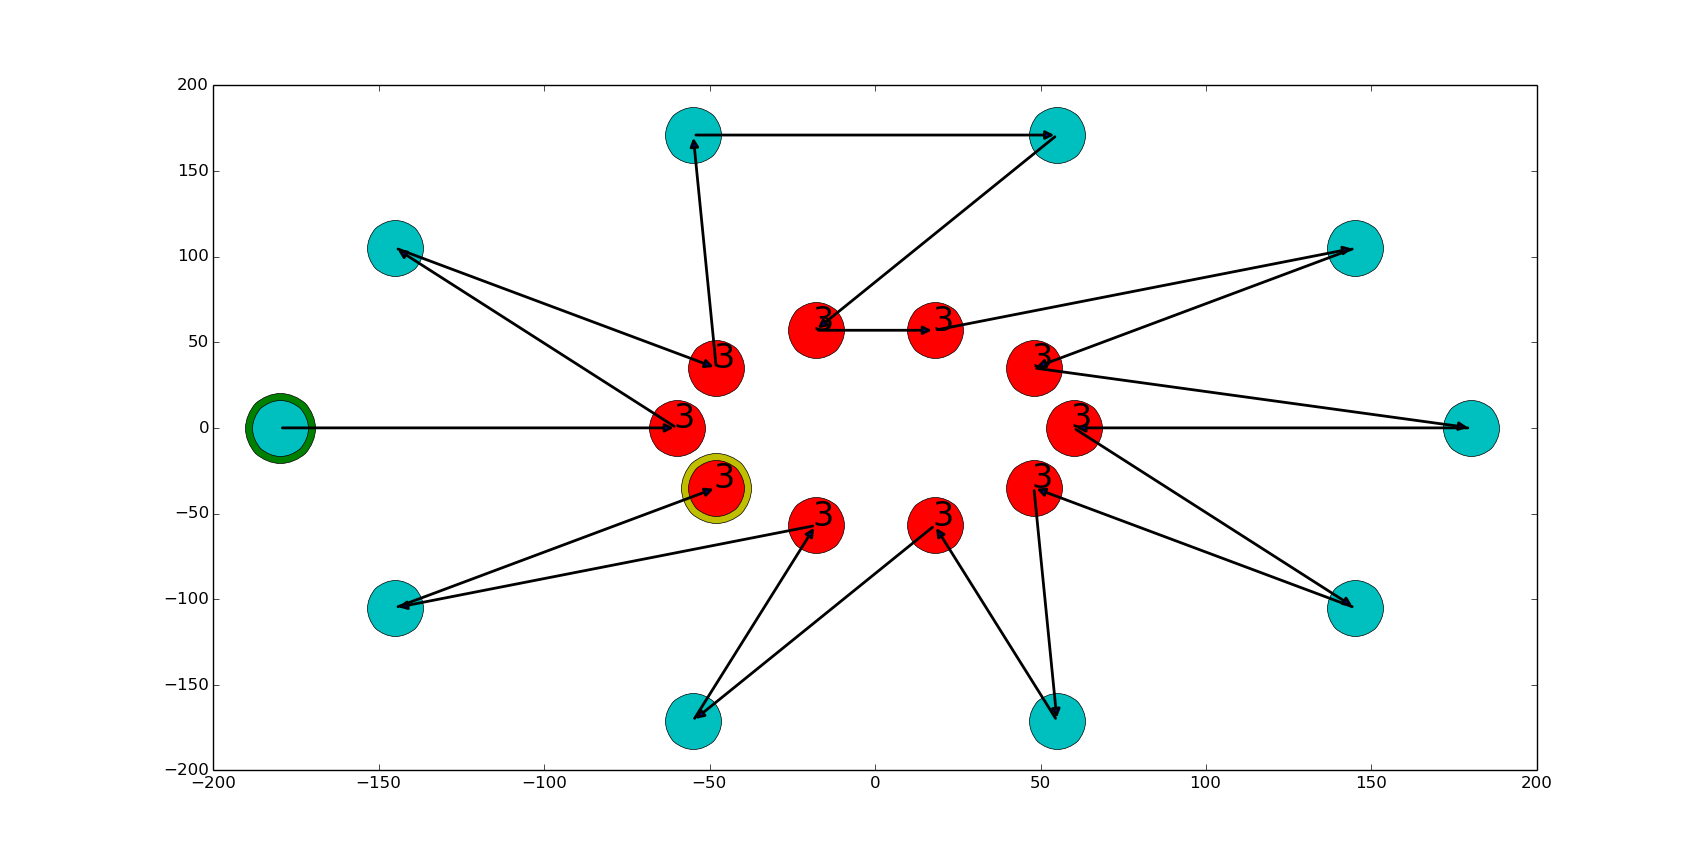
\includegraphics[scale=0.3]{./EJ3/anillos2opt.png}\\
 {            \textit{Soluci\'on 2-OPT}}
  \end{center}
  \vspace*{0.3cm}


\vspace*{0.3cm} \vspace*{0.3cm}
  \begin{center}
 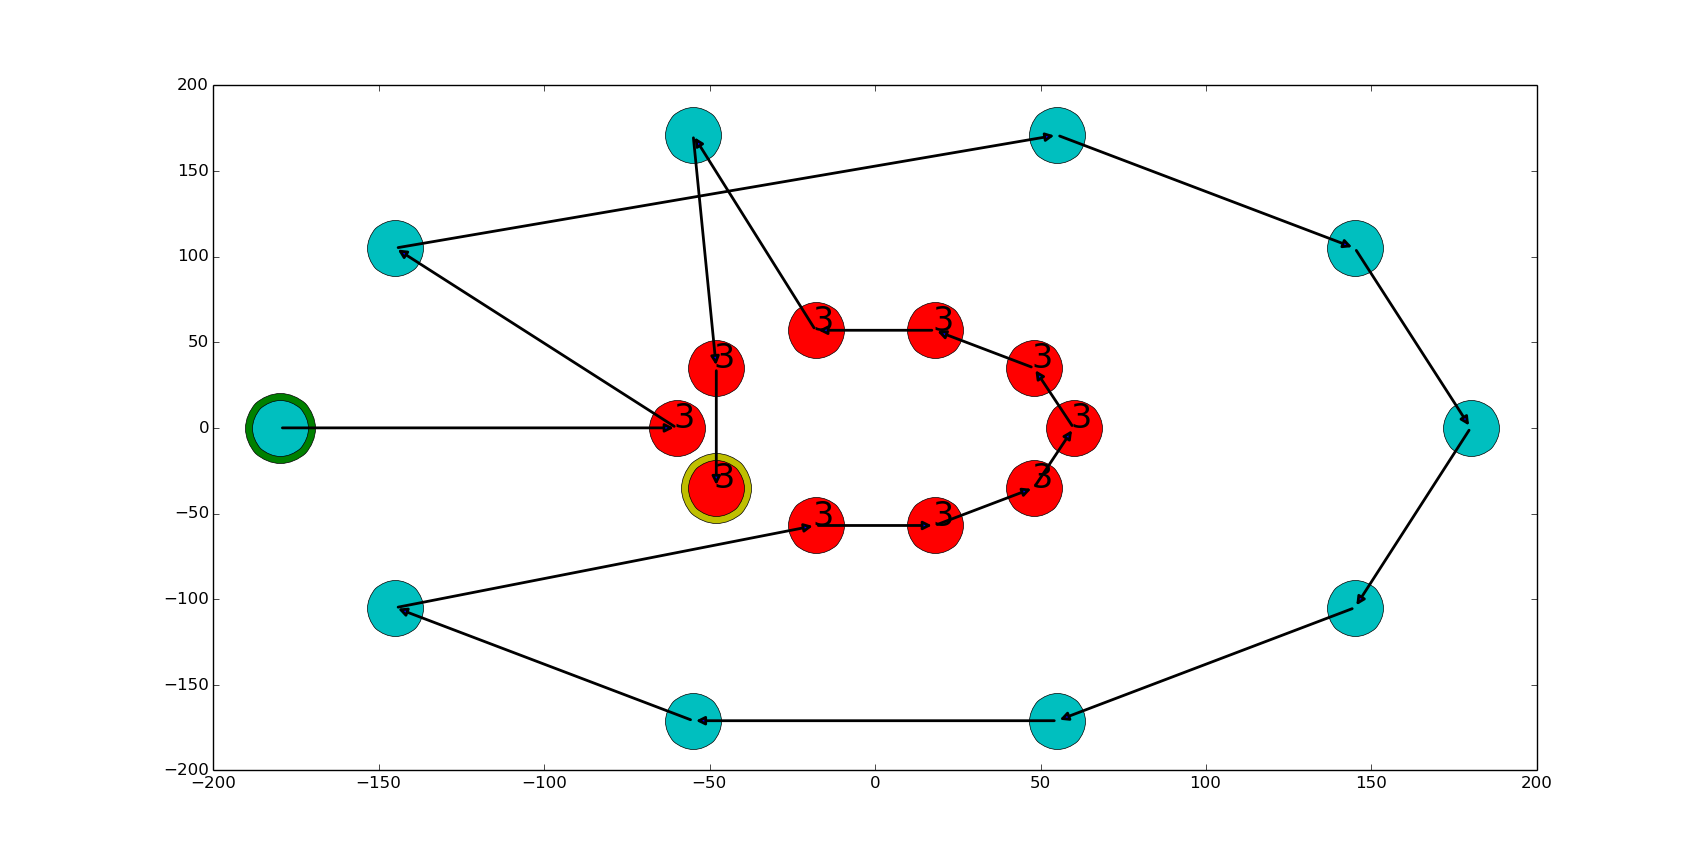
\includegraphics[scale=0.3]{./EJ3/anillos3opt.png}\\
 {            \textit{Soluci\'on 3-OPT}}
  \end{center}
  \vspace*{0.3cm}


  \vspace*{0.3cm} \vspace*{0.3cm}
  \begin{center}
 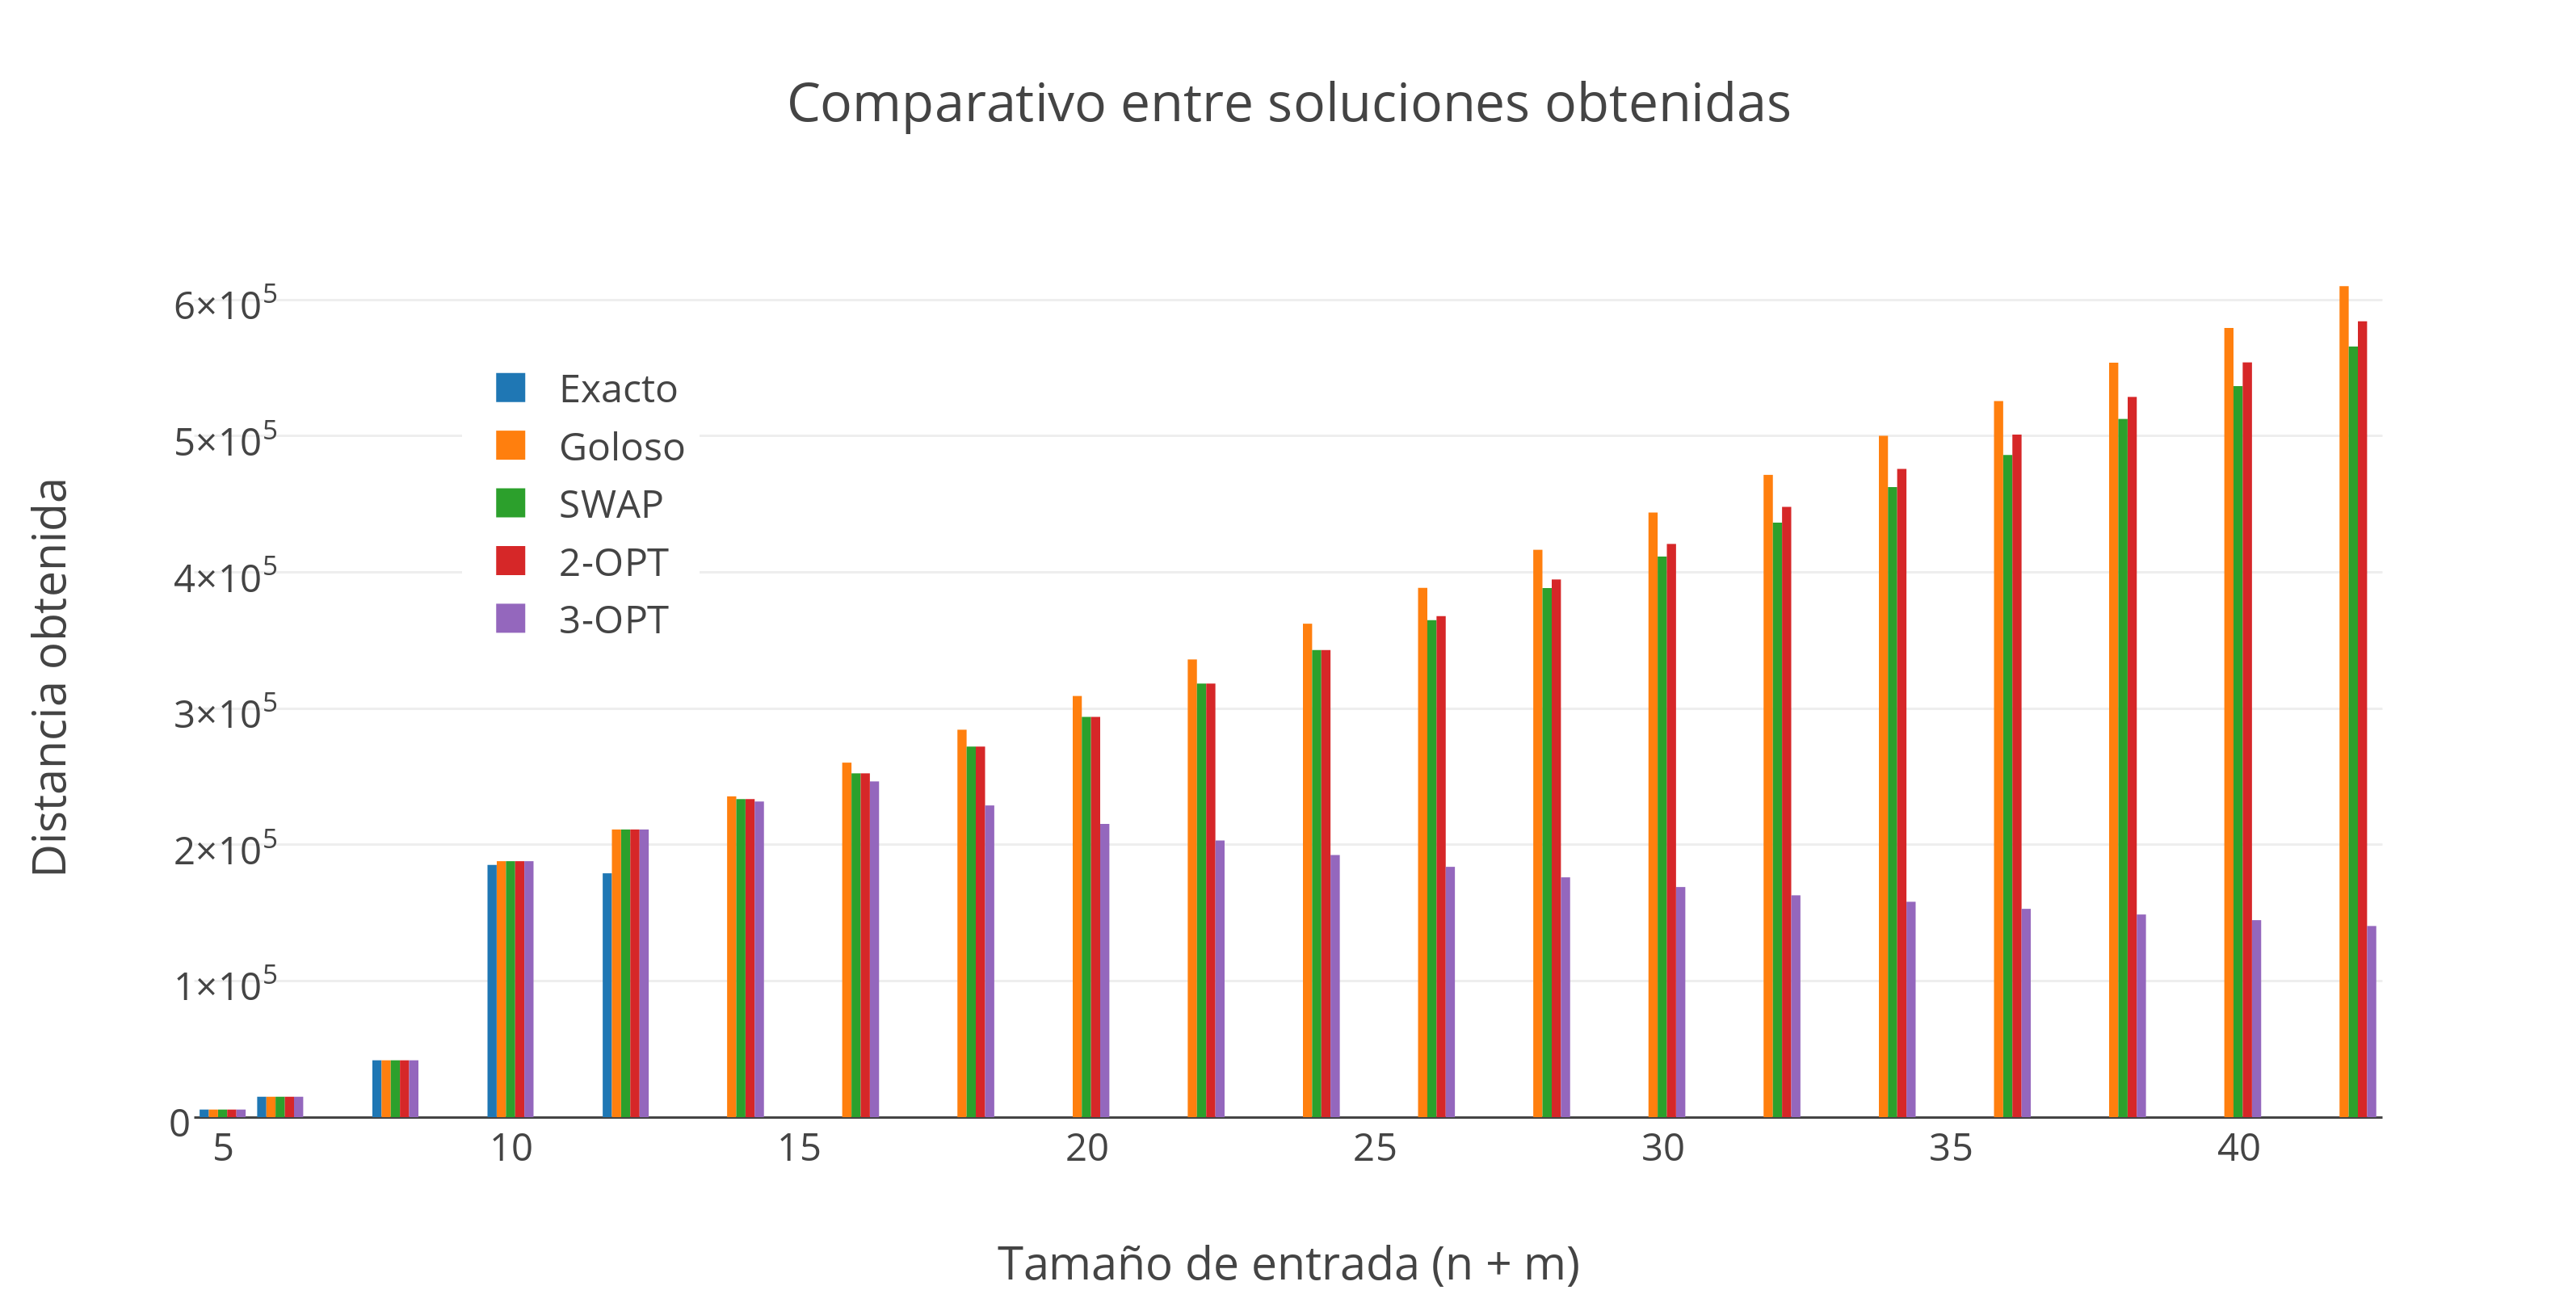
\includegraphics[scale=0.5]{./EJ3/comparacionbusquedaslocalessolucionanillos.png}\\
 {            \textit{Gráfico \ 3.6 - Búsquedas locales sobre Familia 7}}
  \end{center}
  \vspace*{0.3cm}

\vspace*{0.3cm} \vspace*{0.3cm}
  \begin{center}
 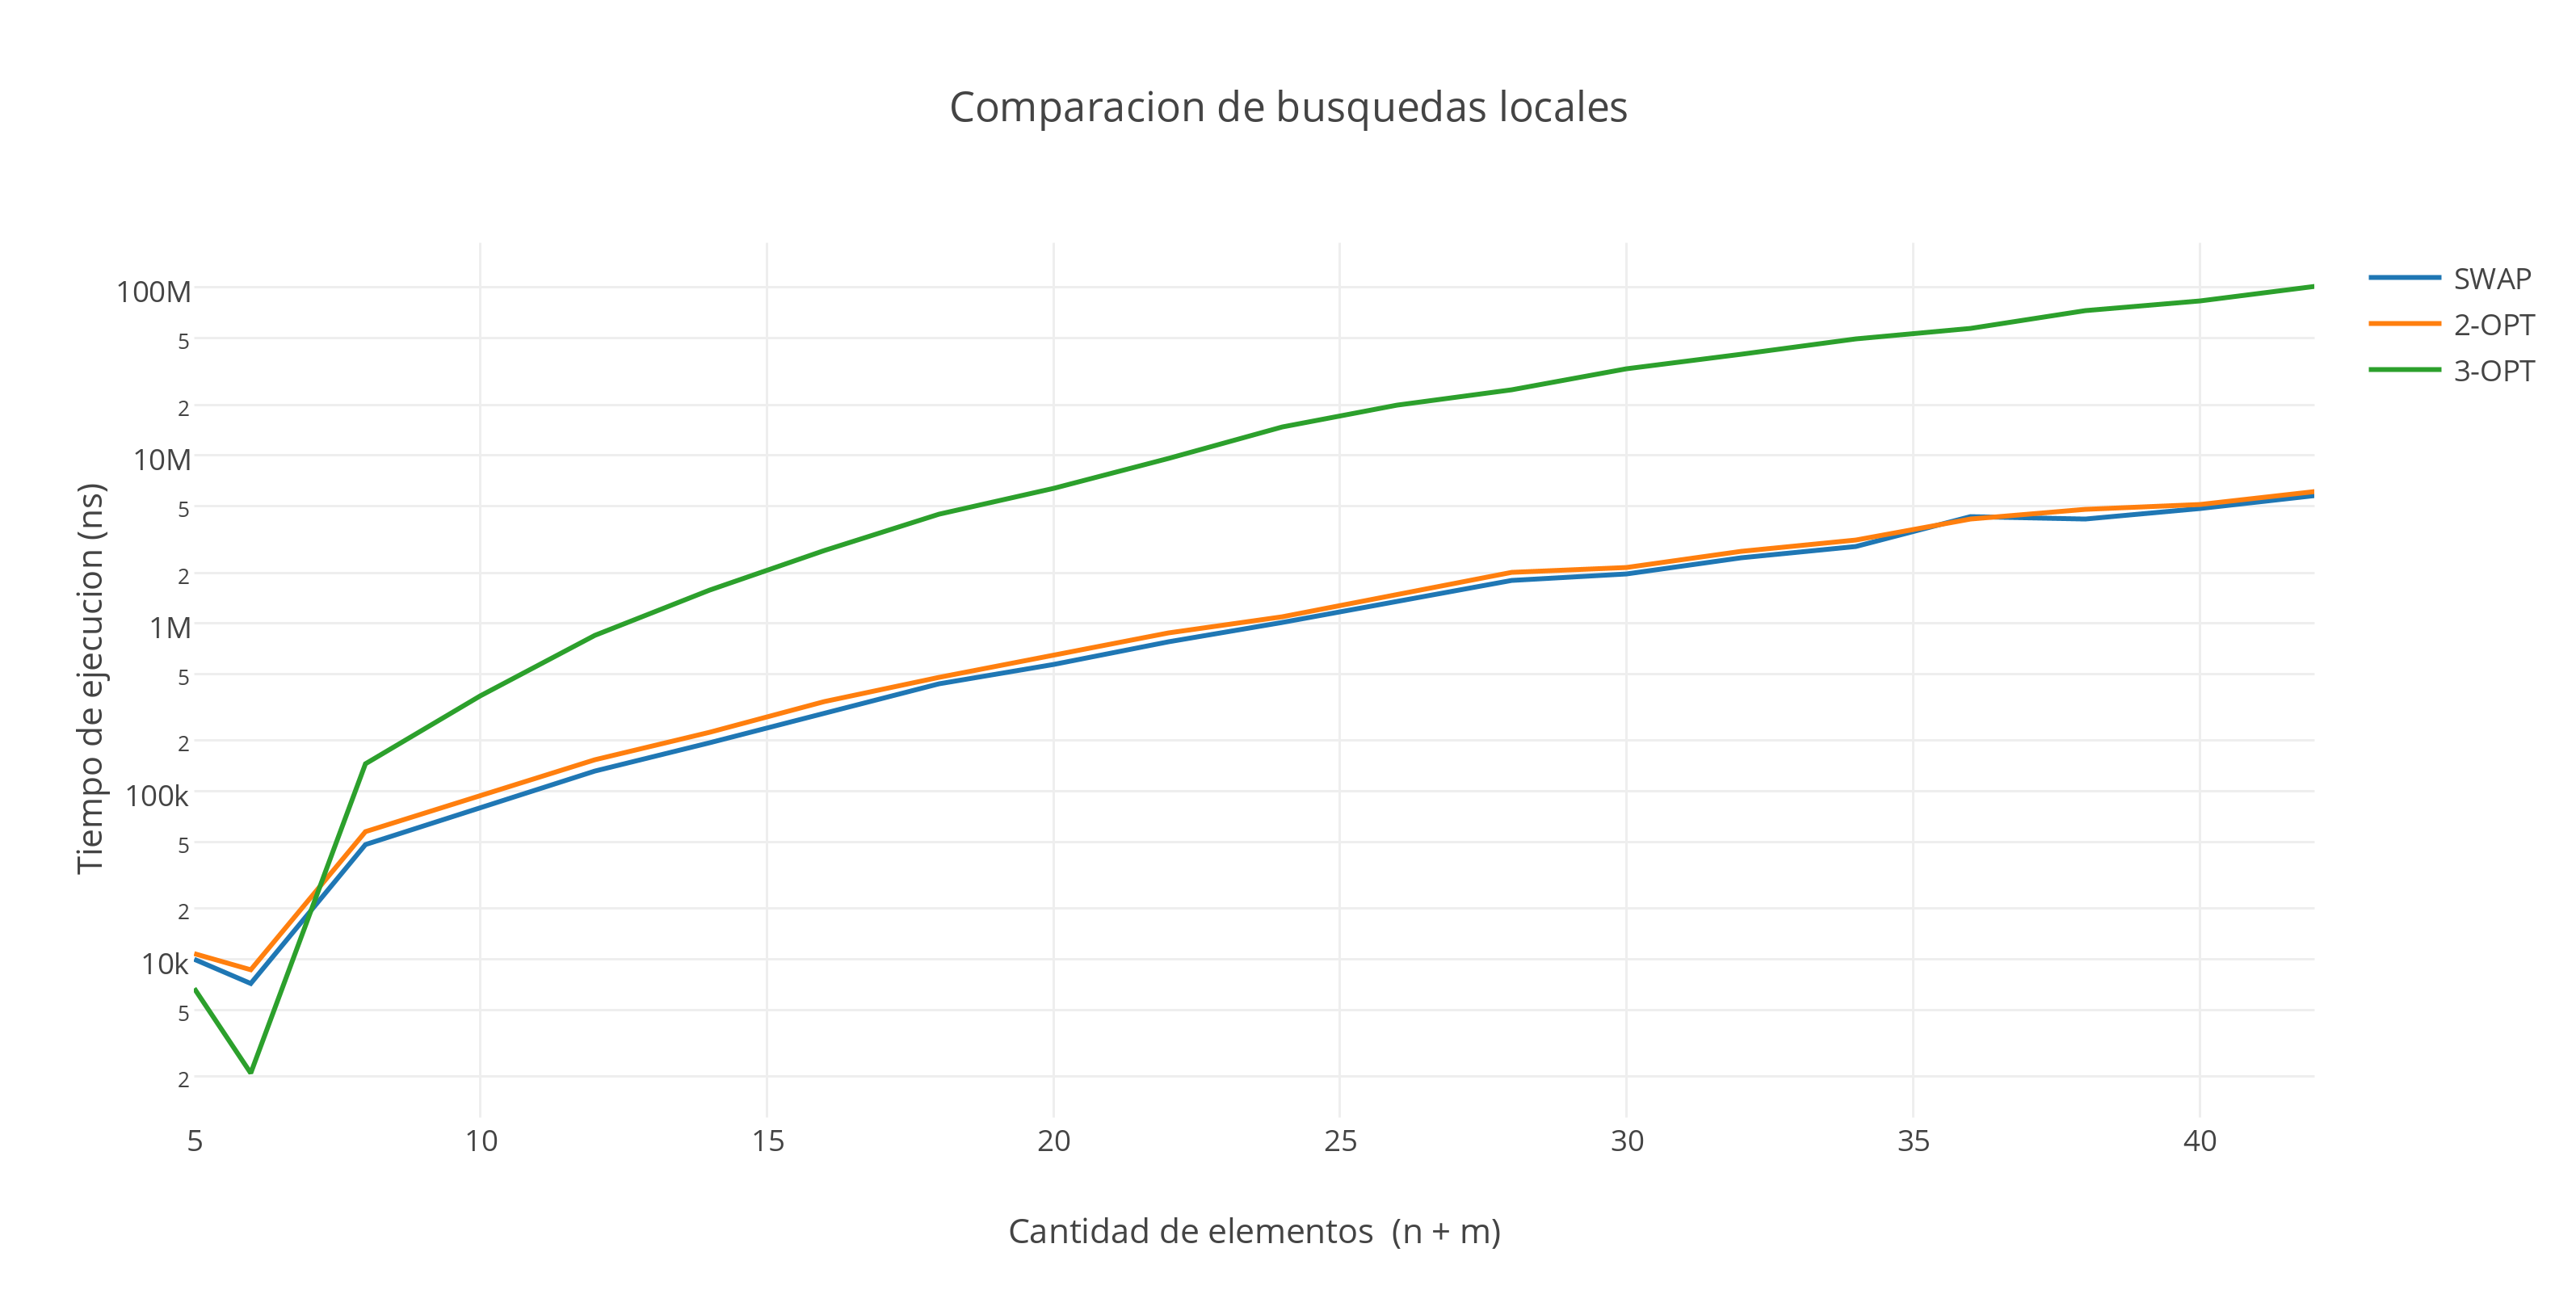
\includegraphics[scale=0.5]{./EJ3/comparacionbusquedaslocalesanillos.png}\\
 {            \textit{Gráfico \ 3.5 - Búsquedas locales sobre Familia 7}}
  \end{center}
  \vspace*{0.3cm}
  
Como sucedió en las familias anteriores, existe una clara diferencia temporal entre 3-OPT y las otras dos búsquedas. En cuanto a la calidad de soluci\'on, podemos ver en este caso que la heur\'istica 3-OPT logra una mejoras superiores en comparación a las otras búsquedas locales. Sin embargo, si se toma en cuenta la relaci\'on tiempo-calidad, debe pagarse un alto costo temporal para obtener estas soluciones.\\
  
\subsubsection*{Familia 8}

Como en las anteriores familias, veremos como se comporta cada heur\'istica para un ejemplo y posteriormente se realizará la comparaci\'on general.

\vspace*{0.3cm} \vspace*{0.3cm}
  \begin{center}
 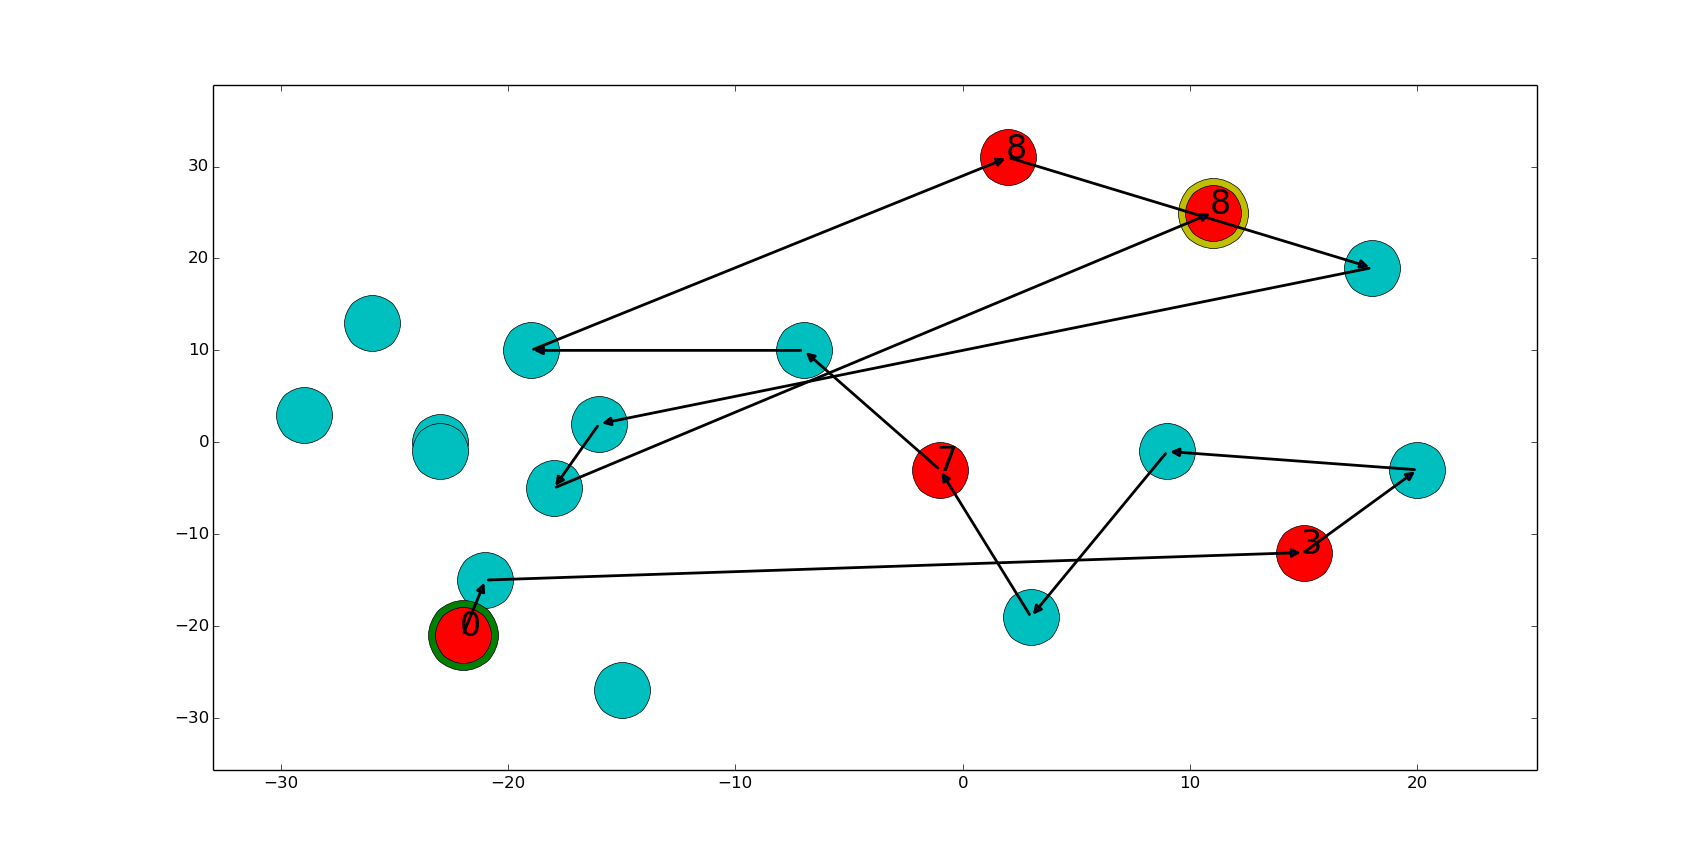
\includegraphics[scale=0.3]{./EJ3/randomgoloso.png}\\
 {            \textit{Soluci\'on Golosa}}
  \end{center}
  \vspace*{0.3cm}

\vspace*{0.3cm} \vspace*{0.3cm}
  \begin{center}
 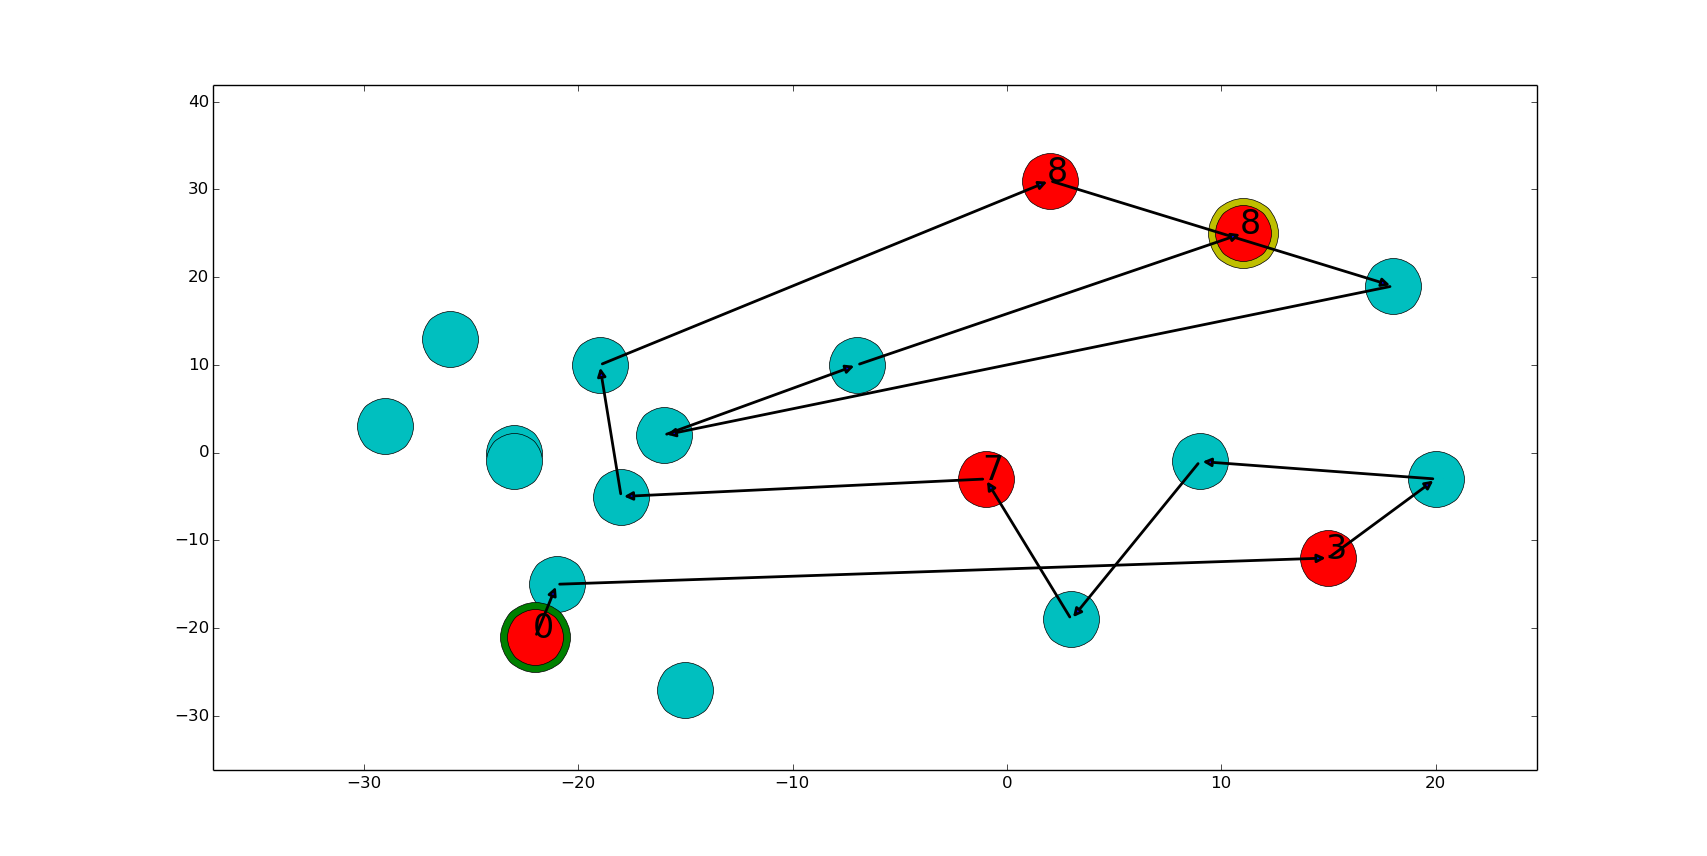
\includegraphics[scale=0.3]{./EJ3/randomswap.png}\\
 {            \textit{Soluci\'on SWAP}}
  \end{center}
  \vspace*{0.3cm}

\vspace*{0.3cm} \vspace*{0.3cm}
  \begin{center}
 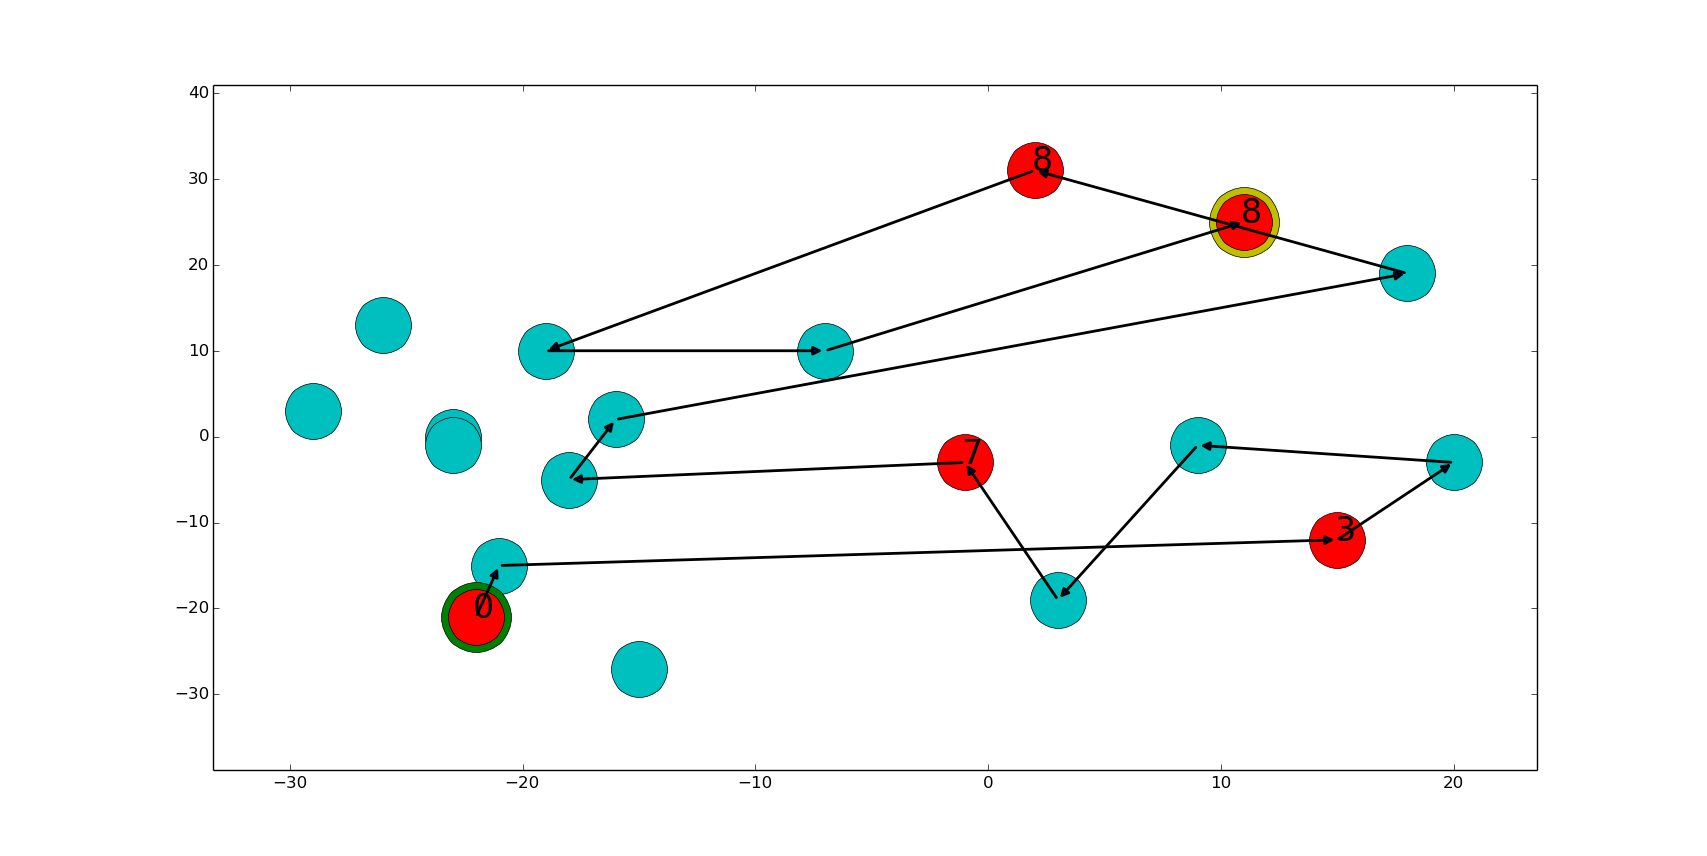
\includegraphics[scale=0.3]{./EJ3/random2opt.png}\\
 {            \textit{Soluci\'on 2-OPT}}
  \end{center}
  \vspace*{0.3cm}


\vspace*{0.3cm} \vspace*{0.3cm}
  \begin{center}
 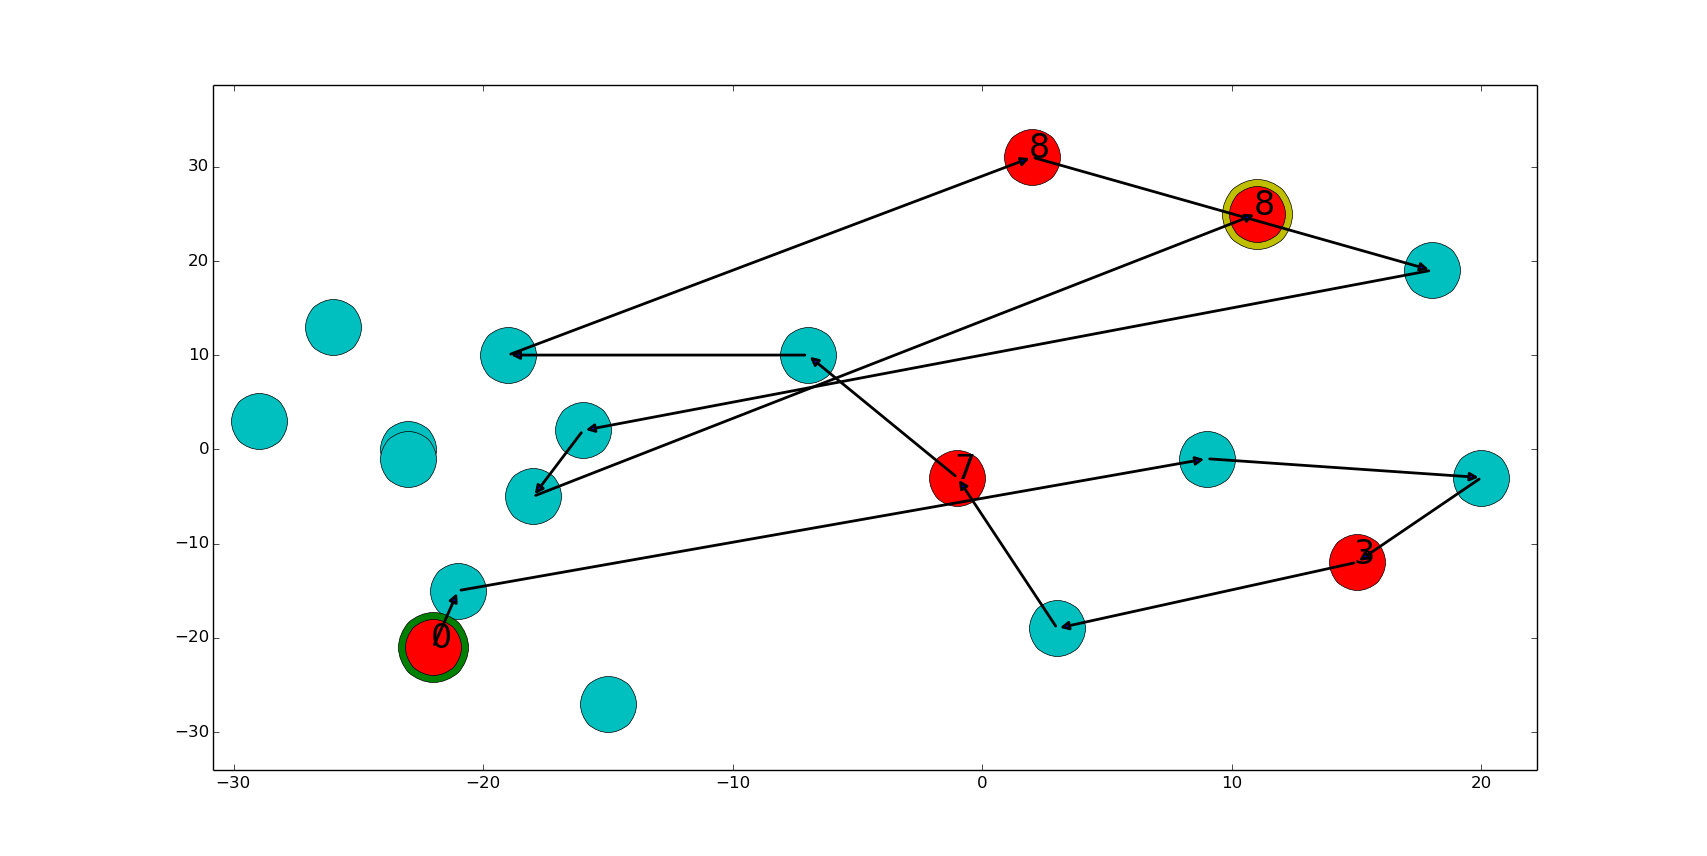
\includegraphics[scale=0.3]{./EJ3/random3opt.png}\\
 {            \textit{Soluci\'on 3-OPT}}
  \end{center}
  \vspace*{0.3cm}
  

\vspace*{0.3cm} \vspace*{0.3cm}
  \begin{center}
 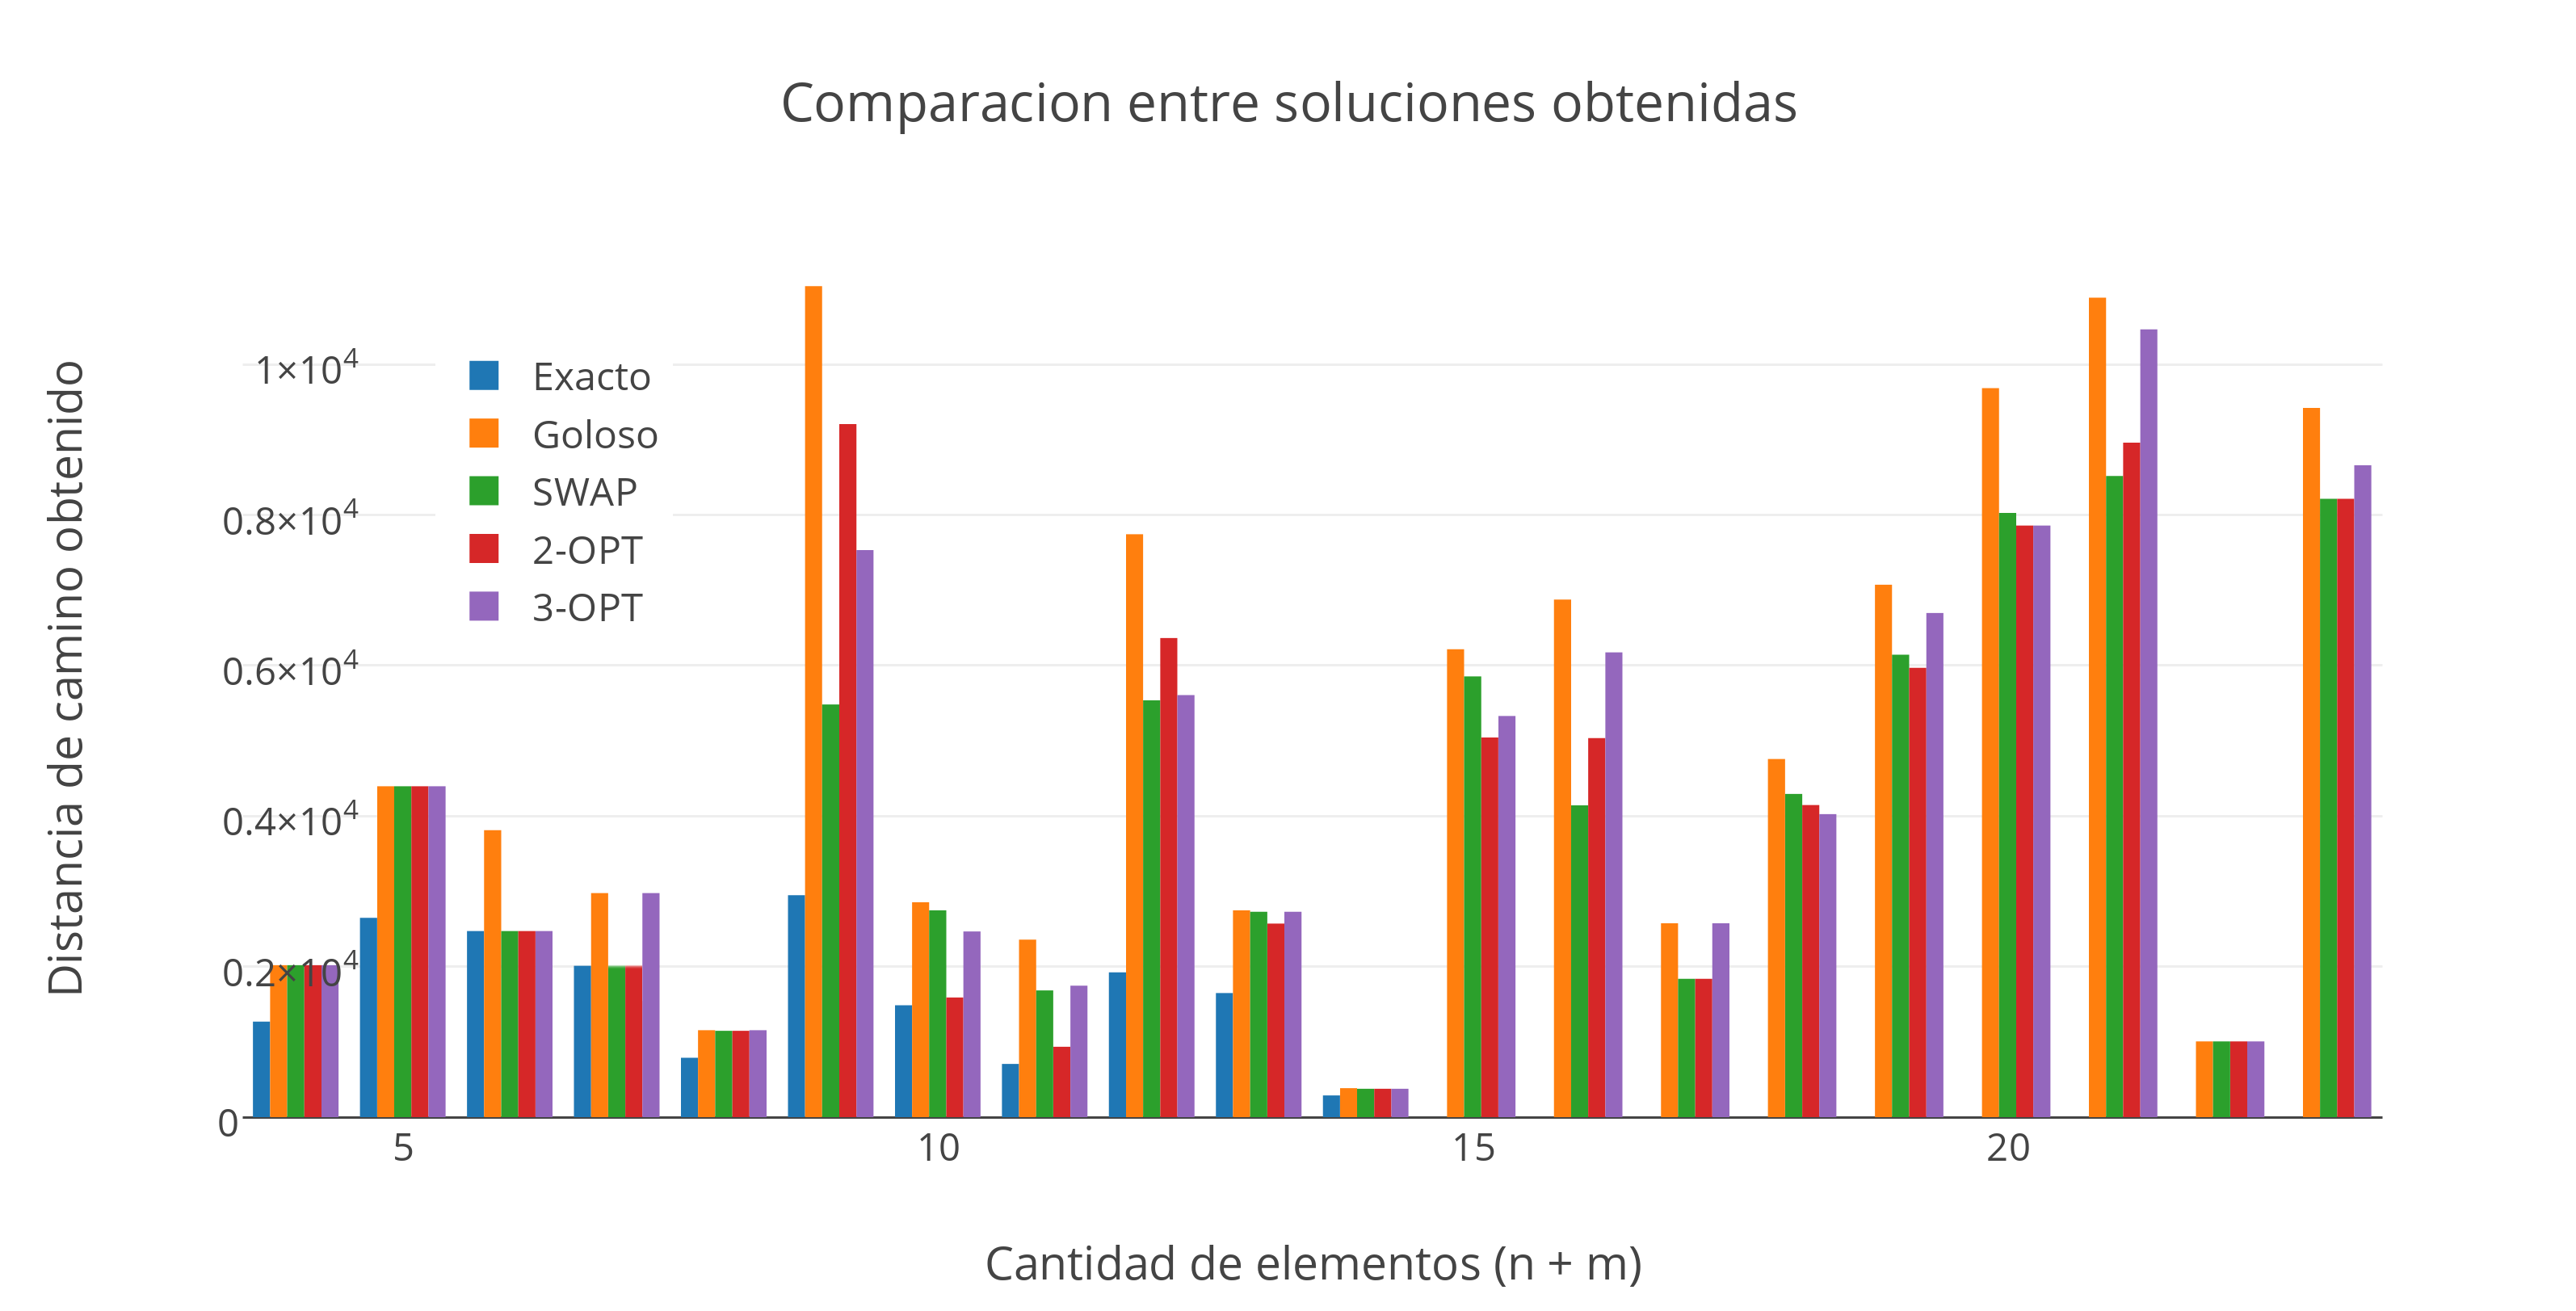
\includegraphics[scale=0.5]{./EJ3/comparacionbusquedaslocalessolucionrandom.png}\\
 {            \textit{Gráfico \ 3.7 - Búsquedas locales sobre Familia 8}}
  \end{center}
  \vspace*{0.3cm}
 
Para este caso se evita la comparación de tiempos debido a que los resultados no ofrecen información relevante que pueda ser analizada comprensivamente, ya que las entradas son de tamaño variable y los tiempos involucrados son muy diferentes.\\

Con respecto a las mejoras obtenidas, los mejores resultados se dividen entre los obtenidos con las búsquedas locales 2-OPT y SWAP.

Podemos considerar que tanto 2-OPT como 3-OPT ofrecen los mejores resultados en cuanto a mejoras se refiere, aunque en el último caso, considerando lo visto en las familias 6 y 7, pagando un alto coste temporal, lo cual puede ser negativo si lo que se busca es mayor velocidad de resolución.

Dado que para entradas mayores a 20 elementos (aproximadamente) obtener resultados exactos es practicamente inviable, siempre que se tiene una solución golosa entre manos y se la optimiza, es complicado saber si se llegó a un óptimo global. Es muy probable que el resultado obtenido de aplicar búsqueda local, sea un mínimo local (de aquí el nombre el algoritmo).\\
Para intentar mejorar los resultados del algoritmo goloso aún más, en el siguiente ejercicio será estudiada una meta heuristica basada en búsqueda local denominada tabú search. La misma trabaja sobre diferentes criterios de búsqueda para ir moviendose entre vecindades e intentar salir de mínimos locales.\\

%Una manera de obtener resultados similares utilizando la misma búsqueda local en este tipo de familias (asumimos que aquel que trabaje con las entradas conoce el tipo de familias al que se enfrenta), podría ser utilizar una condicion de corte diferente donde se finalice la ejecución logrado cierto porcentaje de mejora o si la mejora obtenida en ralación al tiempo insumido no sea considerable.\\
